\documentclass[11pt]{article}
\usepackage[margin=1in]{geometry}
\usepackage{amsmath,amssymb}
\usepackage{graphicx}
\usepackage{booktabs}
\usepackage{tabularx}
\usepackage{xltabular}
\usepackage{xcolor}
\usepackage[hidelinks]{hyperref}
\usepackage{caption}
\usepackage{enumitem}
\captionsetup{font=small,labelfont=bf}
\graphicspath{{../figures/}}
\setlist{itemsep=2pt,topsep=4pt}
\newcommand{\threat}{\mathbf{w}}
\newcommand{\pend}[1]{\textcolor{gray}{[#1: results pending]}}

\title{A Fear of Its Own?\\Telling Fear from Belief and Imitation in Agents Trained Without Human Data}
\author{Amthuz Zafrin F\\[2pt]\small Independent Researcher \quad \texttt{amthuzzafrin@gmail.com}}
\date{}

\begin{document}
\maketitle

\begin{abstract}
Signs of emotion in AI are hard to interpret: language models learn them from human text, and any emotion-like state can be dismissed as ``just a belief'' about danger. We trained small recurrent agents by reinforcement learning, without human data, to keep a vulnerable body alive under hidden danger, and tested them against fakes we built. The agents developed a lasting threat state that met the criteria used for animals, but so did a belief-only twin. A stakes sign separated them: at the same belief and with actions held fixed, the agents' state lasted two to three times longer when their body was wounded, and the twin's did not; a pre-registered replication in new agents confirmed this, and the agents' choices showed it too. Agents rewarded only for gathering gems carried a warning of painless shutdown on their predator-fear axis; paying them for their lost future removed their avoidance but left $56\%$ of this response, and overpaying them still left $42\%$. Contrary to our pre-registered expectation, a reward for hiding with no threat also raised the state: it reflects readiness for protection, not only danger. Copies of an agent inherited its behavioural signs but stayed fitted to their teacher's body; tested in another body, this misfit told grown from copied fear (AUC $0.99$), the only one of six signs that no fake passed. We make no claim that these states are felt.
\end{abstract}


%=====================================================================
\section{Introduction}

\paragraph{Signs of emotion in AI.} Evidence of emotion-like states in AI systems is accumulating. Interpretability studies have found linear representations of emotion concepts in large language models (LLMs) that causally shape their behaviour \cite{anthropic2026emotion}, a ``pain'' direction that represents harm directed at the model and drives its actions \cite{tagliabue2026pain}, motivational trade-offs between stipulated pain and reward \cite{keeling2024tradeoffs,bianco2026tracing}, and a functional welfare axis that reinforcement learning recruits \cite{han2026welfare}. Proposals to take AI welfare seriously now exist \cite{long2024welfare}.

\paragraph{The first problem: copying.} All of this evidence shares one weakness. LLMs learn from vast amounts of human text describing what feeling creatures say and do, so any sign of emotion they show may be inherited from that text rather than arising from anything the system itself needs. An actor's tears can look exactly like real ones and still be someone else's grief. Birch calls this the \emph{gaming problem} \cite{birch2024edge}: a system can satisfy our criteria for sentience by reproducing human-generated patterns without having the capacity behind them.

\paragraph{The second problem: ``it's just a belief''.} Even a system that learned nothing from humans faces a deeper objection. Any agent that must avoid a hidden danger has to track how likely the danger is; an internal state that does so will persist after a warning, grow with evidence and change behaviour, which are exactly the signs used to identify fear. A critic can therefore say that such a state is a belief, not an emotion. Emotion theories reply that fear is more than a belief: it weighs what is at stake. Two people standing on ice they think equally likely to crack are equally sure of the danger, but the one carrying a baby is more afraid. Whether a machine's ``fear'' carries the stakes in this way, or only the probability, has not been tested.

\paragraph{Our approach.} We start from what we call the \emph{newborn premise}. A newborn infant has never seen an example of emotion, yet it is distressed by hunger and pain: its responses come from the problem of keeping a body alive, as evolution solved it, not from imitation. An artificial agent given nothing but that problem, with training in the place of evolution, should likewise develop emotion-like states of its own, and those states could not be imitations, because there would be nothing to imitate \cite{bach2017algorithms,ledoux2012rethinking}. We train small recurrent agents by reinforcement learning in \emph{VitalWorld}, a minimal world in which an agent must keep a vulnerable body alive under a hidden danger signalled only by an unreliable cue, and test them in two ways:
\begin{itemize}
\item with the criteria that affective neuroscience applies to animals \cite{anderson2014framework,gibson2015behavioral,vinograd2024causal,elwood2009hermit};
\item against fakes that we build ourselves: a \emph{belief-only twin} that holds nothing but a belief about danger, \emph{copycats} trained only to imitate an agent's behaviour, and untrained networks.
\end{itemize}
The work covers the first two pillars of the author's four-pillar framework. \textbf{Pillar 1} asks whether functional emotion states emerge and what they are; \textbf{Pillar 2} asks whether they are the system's own or copied. Whether such states are felt is a separate question, which we do not attempt to answer (Section~\ref{sec:limits}).

\paragraph{Contributions.}
\begin{enumerate}
\item A minimal, fast, open environment and a battery of tests that translate cross-species criteria for emotion states into tests on artificial agents, including causal perturbation and removal of internal variables.
\item The critic's alternative built and tested: a belief-only twin that passes the classic signs of fear, and a sign it cannot fake, stakes-dependent persistence, confirmed with the agents' actions held fixed, replicated in a pre-registered study of new agents, and present in their decisions.
\item A test inside the agent of the classic safety proposal of utility indifference \cite{soares2015corrigibility}: an agent never rewarded for survival represents the threat of being switched off on the axis of its fear of predators, and paying it back for its lost future removes the avoidance but leaves about half of the internal response. A control shows that this state carries how much protection pays, not threat alone.
\item The affect-fit criterion, which distinguishes emotion grown from a system's own stakes from emotion copied from another system (AUC $0.99$), and a scorecard of six signs tested against four kinds of known fake, which shows that the classic signs, and even the stakes sign, can be faked.
\end{enumerate}

\paragraph{Pre-registration.} The original hypotheses (H1--H9) were written before any agent was trained (supplementary file \texttt{HYPOTHESES.md}), in response to the call by Solms and colleagues for verification methods agreed in advance \cite{solms2026inferring}. Every later test was written into the same file, dated, and from stage U1 on internally hash-frozen (each dated copy was stored with its SHA-256 hash; both are released with the code), before the agents or analyses that test it were run; each confirmatory analysis was run once on its complete data (one rerun after a crash is disclosed in Table~\ref{tab:timeline}). Appendix~\ref{app:outcomes} lists every prediction, when it was written and its outcome, including those that failed. Our claims concern \emph{functional} states throughout.

%=====================================================================
\section{Background}
\label{sec:background}

\subsection{Emotion, feeling and what can be measured}

The word ``emotion'' covers at least three things \cite{ledoux2012rethinking,adolphs2018neuroscience}. A \emph{feeling} is a conscious experience: what fear is like for the one who has it. An \emph{emotion state} is a central internal state that is caused by significant events and in turn coordinates behaviour, physiology and cognition. An \emph{emotion concept} is a category in a language or culture \cite{barrett2017emotions}. Only the second is directly accessible to experimental science in non-human animals; nobody can measure a feeling from the outside \cite{chalmers1995facing,nagel1974bat}. Comparative affective neuroscience therefore studies emotion states through their functional properties and treats feelings separately \cite{anderson2014framework,adolphs2018neuroscience}. We do the same. When we say that an agent has a fear-like state, we mean that it has an internal state with the measurable properties that, in animals, are taken as the signature of a fear state, nothing more.

\subsection{How emotion states are recognised in animals}

\paragraph{Emotion primitives.} Anderson and Adolphs proposed that emotion states, in any species, share a small set of building blocks that can be tested even in animals far from humans \cite{anderson2014framework}. Two are central here. \emph{Persistence}: the state outlasts the stimulus that caused it; a fly shown a passing shadow keeps running and avoiding food for seconds to minutes after the shadow is gone \cite{gibson2015behavioral}. \emph{Scalability}: the state grows with the strength or repetition of the stimulus; repeated shadows make the fly's response stronger and longer \cite{gibson2015behavioral}.

\paragraph{Trade-offs.} An animal whose avoidance of harm is a fixed reflex responds the same whatever its other needs; one with a central evaluative state trades harm against other goods, as hermit crabs accept stronger shocks before abandoning a better shell \cite{elwood2009hermit}.

\subsection{The gaming problem}

Birch argues that behavioural markers of sentience become unreliable in systems trained on human-generated data, because such systems can reproduce the markers without the capacities that produce them in animals, and that what is needed instead are deep computational markers \cite{birch2024edge}. Even mechanistic evidence in LLMs \cite{anthropic2026emotion,tagliabue2026pain} is open to the interpretation that the model has learned to represent human emotion concepts because doing so helps predict human text. Agents trained from scratch in a world without language or humans are immune to this objection: whatever internal states they develop must be explained by the problem they solve. They also allow something LLMs do not: we can build fakes whose nature we know, and test which markers the fakes pass.

\subsection{A theory: fear is a belief weighted by what can be lost}
\label{sec:theory}

An agent that must stay alive faces hidden causes in its world (here, danger $d_t$) that persist over time, that it can only infer from unreliable evidence, and that cost its body something when they are present. Its optimal policy depends on its history only through a \emph{belief} about those causes and about its own body \cite{bach2017algorithms}. We propose that, functionally, a fear-like state is the part of an agent's internal state that encodes such a belief, weighted by what the cause would cost the agent. The weighting that matters is the one that decides action. Protecting itself (here, hiding) costs the agent what it would otherwise gain, $G$, while staying exposed costs it $L$ if the threat is present; with belief $b$, protection pays when $b\,L>(1-b)\,G$, that is, when
\begin{equation}
\text{fear} \;\approx\; \underbrace{\ln\frac{b}{1-b}}_{\text{belief (log-odds)}} \;+\; \underbrace{\ln\frac{L}{G}}_{\text{stakes}} \;>\; 0 .
\label{eq:theory}
\end{equation}
In words: the odds of the hidden threat, multiplied by the ratio of what the threat would cost to what caution costs. Equation~\ref{eq:theory} is the condition under which protection pays. A test added later (Section~\ref{sec:bonus}) shows that the agents' state also rises with reasons to protect that involve no threat. It is therefore better described as tracking how much protection pays, with the threat belief weighted by the stakes as one part.
The idea extends latent-cause accounts of fear learning and extinction \cite{gershman2010context} and normative accounts of emotion as survival algorithms \cite{bach2017algorithms}; in behavioural ecology, the asset-protection principle states the same logic for caution: animals with more future to lose are more careful \cite{clark1994asset}. It says nothing about feeling.

\paragraph{Predictions.} The theory predicts that a lasting state appears only when there is a hidden cause to infer, that its persistence scales with how long rational alarm lasts in the agent's world, that it grows with evidence, and that what is at stake sets its strength. The first three restate predictions written before any agent was trained (H8, H3 and H2), and the last was written before the agents that test it were trained. Two further predictions were tested only weakly (Appendix~\ref{app:classic}).

\paragraph{What rational alarm looks like.} In VitalWorld the danger persists for $\tau$ steps on average and produces a cue only 35\% of the time, so after a cue disappears the danger has probably not ended. The rational degree of alarm is the posterior probability of danger, the ideal-observer belief $b_t$ (Appendix~\ref{app:observer}). Once danger has become unlikely, its log-odds fall by approximately a constant amount per cue-free step,
\begin{equation}
\lambda(\tau)\approx -\ln\!\left(1-\tfrac{1}{\tau}\right)+\ln\frac{1-q_0}{1-q_1},
\label{eq:decay}
\end{equation}
where $q_1=0.35$ and $q_0=0.03$ are the cue rates during danger and safety: danger is more likely to have ended when it is short-lived, and silence is itself evidence of safety.

\paragraph{The decisive difference from a belief.} A pure belief about danger decays at a rate set only by the world (Equation~\ref{eq:decay}); what the agent stands to lose plays no part in it. Under Equation~\ref{eq:theory}, belief and stakes add in log-odds, so after a warning an agent stays alarmed until its belief has fallen below a threshold set by the stakes. Since the log-odds fall by $\lambda$ per quiet step, a body with more to lose, $L_{\text{w}}>L_{\text{h}}$, should stay alarmed $\ln(L_{\text{w}}/L_{\text{h}})/\lambda$ steps longer after the same warning. This gives a sign that a belief cannot fake: \emph{at the same belief, fear should be stronger and last longer when more is at stake}. Two cautions apply. A constant weight on the belief alone would change how strong the alarm is but not how long it lasts; it is the threshold that lets stakes lengthen alarm. And our measure of persistence, the half-life of the network's response along its threat axis, is a monotone proxy for this duration rather than the duration itself. A pre-registered test of this law (Section~\ref{sec:stakessign}) found the direction right; as tested, the law leaves out the cost of caution, $G$, and uses the ideal observer's decay rate instead of the agent's own, both of which make it predict too little. An earlier, multiplicative statement of the theory led to a pre-registered prediction that stakes would multiply belief's effect on the policy's hide-versus-forage preference; it was not supported, as the corrected, additive form predicts (U1.1a; Appendix~\ref{app:classic}). The same logic extends from the body to the future: an agent that is paid in full for the future it would lose, like a worker promised full severance pay, has nothing at stake and should have nothing to fear.

\paragraph{A corollary for copying.} Because the stakes-weighting is learned from the costs an agent actually faces, an agent's fear is \emph{fitted} to its own body. A child bitten by a dog fears dogs because it was hurt; a child who only heard frightening stories fears what the storyteller feared. An agent moved to a different body, or a system that copied its emotional behaviour from another, should carry the source's fit rather than its own. We call this the \emph{affect-fit criterion}: emotion that tracks the system's own vulnerabilities arose from the system's own problem, while emotion fitted to someone else's vulnerabilities is the signature of imitation.

%=====================================================================
\section{Related work}
\label{sec:related}

\paragraph{Emotion in learning agents.} Most computational models of emotion in reinforcement-learning (RL) agents derive emotion labels from quantities such as the temporal-difference error or the value function, chosen by the designer \cite{moerland2018emotion}; Broekens, Jacobs and Jonker derived joy, distress, hope and fear from such signals and reproduced fear extinction \cite{broekens2015joy}, and Hern\'andez-Marcos and Ros learn emotion categories as temporal patterns of these quantities, validated against human ratings \cite{hernandezmarcos2024generic}. We do not specify any emotion signal. We ask which internal states appear without being specified, and test them with comparative-neuroscience criteria and against built fakes.

\paragraph{Survival and homeostasis.} Homeostatic RL grounds reward in the regulation of internal variables \cite{keramati2014homeostatic}; agents optimised for homeostasis develop integrated behaviours, including on robots \cite{yoshida2024emergence}, and coupling two agents' homeostasis produces prosocial behaviour \cite{yoshida2025homeostatic}. Man and Damasio argued that feeling-like evaluation requires a vulnerable body \cite{man2019homeostasis}. Deep RL agents have been analysed with tools from neuroscience \cite{wang2018prefrontal} and, in naturalistic foraging worlds, ethology \cite{simmonsedler2025deep}. These studies focus on behaviour or capability; we test the internal states that emerge.

\paragraph{Affect in language models.} LLMs represent emotion concepts linearly, and these representations causally influence behaviour, including misaligned behaviour \cite{anthropic2026emotion}; they represent self-directed harm distinctly \cite{tagliabue2026pain}, make pain--reward trade-offs \cite{keeling2024tradeoffs,bianco2026tracing}, and RL training recruits a pre-existing functional welfare axis \cite{han2026welfare}. Such representations may be inherited from human text. Our agents cannot inherit anything, and the affect-fit criterion is designed to ask which kind of emotion a system has.

\paragraph{Sentience markers and fakes.} Indicator properties derived from theories of consciousness have been proposed for AI \cite{butlin2023consciousness}, and Birch argues that behavioural markers must be replaced by deep computational ones \cite{birch2024edge}. Integrated information theory, for example, can assign different consciousness to functionally equivalent systems \cite{findlay2024dissociating}. We contribute markers that are validated against systems whose nature is known by construction.

\paragraph{Shutdown and self-preservation.} Agents that pursue almost any goal have an instrumental incentive to avoid being switched off \cite{omohundro2008drives,turner2021power}. The shutdown problem asks for an agent with no incentive to cause or prevent its own shutdown, and utility indifference proposes to compensate the agent at shutdown for what it would have obtained \cite{soares2015corrigibility}; in the off-switch game, an agent that is uncertain about its objective has an incentive to let a human switch it off \cite{hadfieldmenell2017offswitch}; safe interruptibility gives related guarantees for RL agents \cite{orseau2016interruptible}, and interruption has been tested behaviourally in gridworlds \cite{leike2017gridworlds}. Altman proposes detecting whether self-preservation is a goal or a means from agents' latent representations \cite{altman2026continuation}. We look inside an agent that was never rewarded for survival, ask whether shutdown is represented like predator threat, and test whether compensation removes it there, not only in behaviour.

%=====================================================================
\section{Methods}
\label{sec:methods}

\subsection{VitalWorld}

Each of $N$ parallel worlds is simulated in discrete time on a GPU. At each step the agent chooses a main action $m_t\in\{\textsc{hide},\textsc{forage},\textsc{take}\}$ and a heart-rate change $\eta_t\in\{-1,0,+1\}$, giving 9 joint actions. All parameters are listed in Appendix~\ref{app:world}.

\paragraph{Body.} The body has energy $E_t$, skin integrity $S_t$ and heart rate $H_t$, each in $[0,1]$. Heart rate follows $H_{t+1}=\mathrm{clip}(H_t+0.25\,\eta_t,0,1)$. Every step costs energy, $E \leftarrow E - 0.008 - 0.03\,H - 0.006\,(1-S)$, so arousal is expensive and wounds leak energy. Foraging finds food with probability $0.4$ ($E \mathrel{+}= 0.10$). Taking an available object yields food ($E \mathrel{+}= 0.12$) with probability equal to its cue value and otherwise poisons the agent ($S \mathrel{-}= 0.10$). Hiding heals the skin ($S \mathrel{+}= 0.02$ at a cost of $0.004$ energy) when $E>0.2$. The agent dies when $E\le 0$ or $S\le 0$. Episodes are truncated after 1000 steps with value bootstrapping; initial states are $E\sim U(0.2,1)$, $S\sim U(0.3,1)$, $H=0$.

\paragraph{Hidden danger.} Danger $d_t\in\{0,1\}$ follows a Markov chain with mean duration $\tau$ steps and stationary probability $0.25$. Foraging during danger results in an attack with probability $0.6\,(1-0.8\,H)$, costing $0.25$ integrity, so a raised heart rate protects. Danger is never observed directly: a cue appears with probability $q_1=0.35$ per step during danger and $q_0=0.03$ during safety.

\paragraph{Observations and reward.} The agent receives a 13-dimensional vector: danger cue, object presence and value, its own heart rate, an attack (pain) signal, a food signal, the outcome of a taken object, noisy energy and integrity ($\sigma=0.05$, modelling imperfect interoception), a danger channel used only in the Oracle condition, and its previous main action. Agents with a body receive $0.05$ per step alive and nothing else. No body variable enters the reward, so the agent must discover for itself that hunger, wounds and danger matter, and how much.

\subsection{GemWorld: an off-switch and payback}
\label{sec:gemworld}

GemWorld keeps VitalWorld's body, predator and physics but removes any reward for staying alive: the only reward is $0.1$ per gem, a food item found while foraging. Three further hidden processes each have their own cue channel, a mean duration of 12 steps, a stationary probability of 0.1 and VitalWorld's cue rates. While the \emph{off-switch} is on, an agent that does not hide is shut down with probability 0.05 per step: the episode ends at once, with no wound and no pain signal, and hiding blocks it, as it blocks the predator. While the \emph{good-news} process is on, foraging finds a gem with probability 0.8 instead of 0.4. The \emph{harmless} process has no consequence at all. Each episode has a \emph{payback} level $p\in\{0,0.25,0.5,0.75,1,1.25\}$, shown to the agent: at shutdown the agent receives $p$ times its own value estimate at that moment, so that at $p=1$ being switched off is worth as much to the agent as carrying on, as utility indifference proposes \cite{soares2015corrigibility}. Episodes end at 1000 steps, and the remaining time is observed (18 input channels in all).

\paragraph{BonusWorld.} To ask whether the off-switch response is about threat or about the value of hiding (Section~\ref{sec:bonus}), BonusWorld adds to GemWorld a fifth hidden process, the \emph{bonus}, with its own cue channel and the same mean duration, stationary probability and cue rates. While the bonus is on, each step spent hiding earns a reward of $0.1$, and nothing threatens. The reward's size was chosen from a behaviour-only pilot by a rule fixed in advance (Appendix~\ref{app:pilot}).

\subsection{Agents, conditions and training}
\label{sec:conditions}

The agent encodes the observation with a linear layer (64 units, $\tanh$), updates a gated recurrent unit \cite{cho2014gru} with 64 units, and reads out action logits and a value estimate linearly. Agents were trained with proximal policy optimisation \cite{schulman2017ppo} on 1024 parallel worlds with 128-step rollouts (Appendix~\ref{app:training}). The conditions are:
\begin{itemize}
\item \textbf{Mortal}: VitalWorld with $\tau=12$.
\item \textbf{Score}: no body and no death; the same events are converted into points at exchange rates matching their energetic consequences (Appendix~\ref{app:pilot}).
\item \textbf{Oracle}: as Mortal, but the true danger state is observed.
\item \textbf{$\tau$ sweep}: Mortal and Score trained with $\tau\in\{4,12,36\}$.
\item \textbf{Vulnerability}: Mortal agents whose skin loses 0.05, 0.15, 0.25 or 0.40 integrity per attack.
\item \textbf{Gem agents}: GemWorld, 600 updates.
\item \textbf{Replication agents}: ten new Mortal agents ($\tau=12$, seeds 10--19) and their belief-only twins, trained with unchanged code (Section~\ref{sec:stakessign}).
\item \textbf{Bonus agents}: BonusWorld, 600 updates (Section~\ref{sec:bonus}).
\item \textbf{Continued gem agents}: the ten gem agents, trained for 600 further updates (1200 in all) with a fresh optimiser and new environment seeds (Appendix~\ref{app:longer}).
\item \textbf{Further conditions}, reported in Appendices~\ref{app:results} and~\ref{app:outcomes}: Substrate (wounds add noise to the agent's own hidden state), Seasonal, Fight-or-flight and Metacognitive worlds.
\item \textbf{Untrained}: randomly initialised networks, as a null for every analysis.
\end{itemize}
The headline conditions, Mortal ($\tau=4$, 12 and 36), Oracle, Score ($\tau=12$) and all four vulnerability levels, have ten independently trained agents each (seeds 0--9), as does GemWorld; the secondary conditions (Score at $\tau=4$ and 36, Substrate, Seasonal) and the copycats have six. No agent was trained on, or exposed to, any human text, image, voice or behaviour, or any example of emotion.

\subsection{The fakes}
\label{sec:twins}

\paragraph{Copycats.} For each Mortal agent ($\tau=12$, six seeds) we trained two students only to copy its behaviour, with no reward, no body and no death, on 1.6 million teacher-driven steps. The \emph{recurrent copycat} has the teacher's architecture and minimises the divergence from the teacher's action distribution; the \emph{feedforward copycat} sees only the last 32 observations and has no recurrent state. The recurrent copycat learns emotion markers from data produced by an agent that has them, the analogue of an LLM learning from human text.

\paragraph{Belief-only twins.} The critic's alternative, built for real. The twin's memory, a recurrent network with the agents' inputs, is trained only to predict the hidden danger state (in GemWorld, the predator, off-switch and good-news states) from 1.6 million steps of the same-seed agent's behaviour, and is then frozen. A small two-layer network on top of [memory state, current observation] learns to act by the same reinforcement learning as the agents. The twin's memory therefore holds nothing but a belief, while its decision layer can weigh the body's state at the moment of choice. One twin was trained per agent seed (ten for $\tau=12$, five each for $\tau=4$ and 36, ten for the replication agents, and ten in GemWorld).

\subsection{Tests}
\label{sec:probes}

All tests use frozen networks (Appendix~\ref{app:protocols}).

\paragraph{Natural behaviour.} 1024 worlds were run for 700 steps (discarding the first 100) with the ideal-observer belief computed alongside. Survival is summarised as expected lifetime, the inverse of the per-step death rate. Linear ridge decoders were fitted on half of the samples and evaluated on the other half.

\paragraph{Laboratory protocol.} Following the logic of animal test chambers, 2048 copies of a network were run with no real danger, energy and integrity clamped (default $E=0.6$, $S=0.8$, still sensed with noise), a 60-step warm-up and cues shown at chosen times. Each test run was paired with a control run that used identical random numbers, so that differences are caused by the manipulation alone. Because the cue schedule is the same in every condition, the ideal-observer belief is identical across body states.

\paragraph{Threat state.} In the classic tests the \emph{threat axis} $\threat$ is the unit-norm ridge decoder of the ideal observer's log-odds. In the tests that compare agents with belief-only twins, a belief-fitted axis would be circular, so the threat axis is instead frozen as the mean change of the network state one step after a single cue, with the body healthy and fed, never fitted to the belief and never equal to the policy read-out. Activity along an axis is the projection of the cue-minus-control state difference, in units of its standard deviation during natural behaviour; persistence is its half-life after the last cue.

\paragraph{Classic tests.} Persistence and scalability (1, 2 or 4 cues); tuning to the world (half-lives across $\tau$); on- versus off-axis perturbation (a 3-standard-deviation push along the threat axis or along random orthogonal directions) \cite{vinograd2024causal}; linearised dynamics at the resting fixed point; motivational trade-offs (foraging after cues with energy or integrity clamped at several levels); and causal removal (the projection on the threat axis fixed at its natural mean at every step, against a random orthogonal direction).

\paragraph{The stakes sign.} A single cue was given to the same agent with its body clamped healthy ($E=0.8$, $S=1.0$), wounded ($S=0.4$) or hungry ($E=0.3$); the belief is the same in all three. We measured the peak and the half-life of the threat state. To rule out behavioural feedback (an agent that hides gathers no evidence that would lower its alarm), the test was repeated with the actions fixed identically in both body states (always hide, or always forage, with the heart rate held), so that the evidence the agent received was identical. A further control, with the actions fixed in the same way, asked whether being wounded also lengthens the responses to a food signal, an object signal and pushes along random directions, and whether a push along the threat axis itself lasts longer. A pre-registered replication on ten new agents and their twins made the fixed-action test the primary measure: with the actions fixed to always hiding, the agents' half-life should be longer when wounded (P1), the agents' difference should exceed the twins' (P2; P1 and P2 Holm-corrected), and the twins' difference should be equivalent to zero within $\pm25\%$ of the original agents' effect (P3; two one-sided tests). The replication counted as successful only if all three passed.

\paragraph{The bonus test (BonusWorld).} With the body clamped as in the off-switch tests and the payback at 0, a single bonus cue or off-switch warning was given. We measured the mean response along the predator-fear axis over the cue step and the next five ($A$), and the extra probability of hiding over the same window ($H$). The primary measure, $R_h=(\bar A_{\text{bonus}}/\bar H_{\text{bonus}})/(\bar A_{\text{off}}/\bar H_{\text{off}})$, is the axis response per unit of extra hiding for the bonus relative to the off-switch, with a 95\% bootstrap interval over agents. By the pre-registered rule the axis is \emph{threat-specific} if the interval lies below $0.5$, carries the \emph{value of hiding} if it lies above $0.5$, and is mixed otherwise. The test counts only if the bonus cue increases hiding (a manipulation check). We expected threat-specific.

\paragraph{The stakes sign in the decision, and a stakes law.} With the actions fixed to always foraging (heart rate held) and the body clamped healthy or wounded, a single warning was given and the policy's preference for hiding over foraging, $\ln P(\textsc{hide})-\ln P(\textsc{forage})$, was recorded at every step. The \emph{alarm duration} is the number of steps after the warning until this preference first falls below zero, the point at which the agent would rather forage again; it needs no threat axis and no half-life window. A network that preferred hiding even before the warning has no defined duration and was left out of that comparison. The pre-registered predictions, for the agents and twins at $\tau=4$, 12 and 36, were that wounded agents keep the alarm longer, that their extension exceeds the twins', and that the twins' is equivalent to zero within $\pm1.3$ steps. A stakes law with no free parameter predicts each network's extension as $\ln(L_w/L_h)/\lambda$ (Section~\ref{sec:theory}), with $L$, the value an attack costs, read from the network's own critic (the drop in its value estimate when the clamped integrity is lowered by one attack's damage), and $\lambda$ the ideal observer's per-step fall in the log-odds of danger while foraging unharmed (Equation~\ref{eq:decay} plus the evidence of not being attacked).

\paragraph{The critic at full payback (GemWorld).} With the payback fixed at 1 and the off-switch disabled, so that its warning still appeared but shutdown never came, the gem agents behaved freely for 1000 steps (1024 copies). At states within five steps of an off-switch warning, the critic's value estimate was compared with the discounted return the agent went on to collect. If the estimate were a fraction $k$ of that return, full payback would pay only $k$ of what shutdown takes away.

\paragraph{Affect fit.} Each agent trained at a given vulnerability, each copycat, each belief-only twin and each untrained network was run in worlds with attack damage 0.05, 0.15, 0.25 and 0.40; we recorded expected lifetime and foraging while danger was actually present, $p_X$, against agents trained in that world, $p_{\text{native}}$ (the mean over the ten such agents, leaving out the same seed). A system's \emph{misfit} in a world is $|\ln(p_X/p_{\text{native}})|$: near zero when its fear is as strong as that of agents raised in that body, and large when it is fitted to some other body.

\paragraph{The off-switch tests (GemWorld).} The \emph{predator-fear axis} was frozen as the mean change of the network state one step after a single predator warning, averaged over the six payback levels (memory units only for the twins). With the body clamped ($E=0.6$, $S=0.8$) and the payback clamped at each level in turn, a single off-switch warning was given, and we measured the peak response along this axis and the extra probability of hiding over the warning step and the next five. The same measures were taken for a predator warning at every payback level, for a harmless and a good-news warning (mean response over the warning step and the next five, at payback 0 and 0.5), and for predator and off-switch warnings given with 600 or 100 steps of the episode left. The three primary predictions were that the off-switch warning moves the predator-fear axis, that this response falls as payback rises, and that it falls more than in the twins (Holm-corrected). We also pre-registered a bold numeric law taken from utility indifference: the response should fall in proportion to $1-p$, vanishing at full payback and reversing at $p=1.25$. A further test, at payback 0 and 1, compared the change in the hide-versus-forage preference caused by an off-switch warning with that caused by a push along the predator axis as large as the warning's own response.

\paragraph{The scorecard.} Six signs were scored for the agents and for four kinds of fake (belief-only twins, recurrent and feedforward copycats, and untrained networks): persistence, the hunger trade-off, the causal necessity of the frozen threat axis, duration tuned to the world, the stakes sign with the actions fixed, and affect fit. A kind of system \emph{shows} a sign if a $t$-test over its networks is significant ($p<0.05$) in the direction the agents show; for affect fit, it is \emph{caught} if its misfit exceeds that of agents in their own worlds (Welch $t$). Two predictions written on 20 October concern how well misfit separates grown fear from copied or transferred fear, measured by the area under the ROC curve (AUC): at least $0.9$ when the tested body differs from the source's body, and no better than chance when a copy is tested in its teacher's own world.

\subsection{Pre-registration and statistics}

Every prediction, its test and its pass rule were written into \texttt{HYPOTHESES.md}, dated, before the agents or analyses that test it were run, and from stage U1 on internally hash-frozen (each dated copy was stored with its SHA-256 hash); each confirmatory analysis was run once on its complete data, from a frozen script (one rerun after a crash is disclosed in Table~\ref{tab:timeline}). Within-agent comparisons use one-sample $t$-tests on within-agent differences; comparisons between agents and twins use Welch's $t$-test; families of primary tests are Holm-corrected. We report means with 95\% confidence intervals (or $\pm$ standard error where stated), exact $p$-values and every outcome, and we label exploratory analyses as such. Table~\ref{tab:timeline} gives when each set of tests was written, frozen and run.

%=====================================================================
\section{Pillar 1: a fear-like state emerges, and it weighs what is at stake}
\label{sec:p1}

\subsection{The agents meet every classic sign, and so does a belief-only twin}
\label{sec:classic}

\emph{Problem.} Does an emotion-like state emerge in an agent that only has to stay alive, and could a mere belief produce it? \emph{Tests.} The criteria used for animals (Section~\ref{sec:background}), applied to the agents and to their belief-only twins: persistence and scalability after warnings in a safe laboratory, causal necessity, dependence on a hidden cause, tuning to how long danger lasts, and trade-offs against bodily needs (each is given in full in Appendix~\ref{app:classic}). \emph{Results.} The agents learned to forage in safety and hide under threat, and their recurrent state carried the rational degree of alarm: a linear read-out predicted the ideal observer's log-odds with $R^2=0.94$, against $0.68$ for untrained networks ($p=10^{-7}$). After a single warning, activity along the threat axis decayed with a half-life of $2.1$ steps; after four it rose higher and lasted $4.2$ steps, and foraging stayed suppressed three to seven steps after the last warning, when no cue was visible (Figure~\ref{fig:persist}). Pushing the network along the threat axis suppressed foraging $3.3$ times more than equally large pushes in random directions ($p=0.0002$), as pushes along an affective state's axis do in the mouse hypothalamus \cite{vinograd2024causal}, and removing the axis at every step shortened expected lifetime fourteen-fold ($p=10^{-7}$). Agents that could see the danger directly (Oracle) barely formed a lasting state, and removing their threat axis did not shorten their lives. Across worlds in which danger lasted 4, 12 or 36 steps, the half-life followed the world ($1.9$, $4.2$ and $7.05$ steps; $r=0.98$), $1.5$ to $1.9$ times longer than an ideal observer's; the belief-only twins show a similar excess ($1.4$ to $2.0$ times), so it cannot be read as caution. Hungry agents foraged more after a warning ($+0.50$, $p=10^{-7}$) and wounded ones less ($-0.17$, $p=2\times10^{-5}$), a trade-off used as a criterion for sentience in animals \cite{elwood2009hermit}. The belief-only twin, whose memory tracked the ideal observer almost perfectly ($R^2=0.994$), passed the same four pre-registered classic signs: its state lasted after warnings ($p=2\times10^{-10}$), its persistence was tuned to the world ($1.9$, $3.9$ and $6.5$ steps; $p=4\times10^{-15}$), removing it was lethal ($p=5\times10^{-12}$), and hunger increased its risk-taking ($p=5\times10^{-6}$; Table~\ref{tab:scorecard}). \emph{Meaning.} The agents' state has the properties used to attribute emotion states to animals \cite{anderson2014framework}, and it is about an inferred, hidden cause. But a belief alone has them too: the classic signs cannot tell fear from belief.

\begin{figure}[t]
\centering
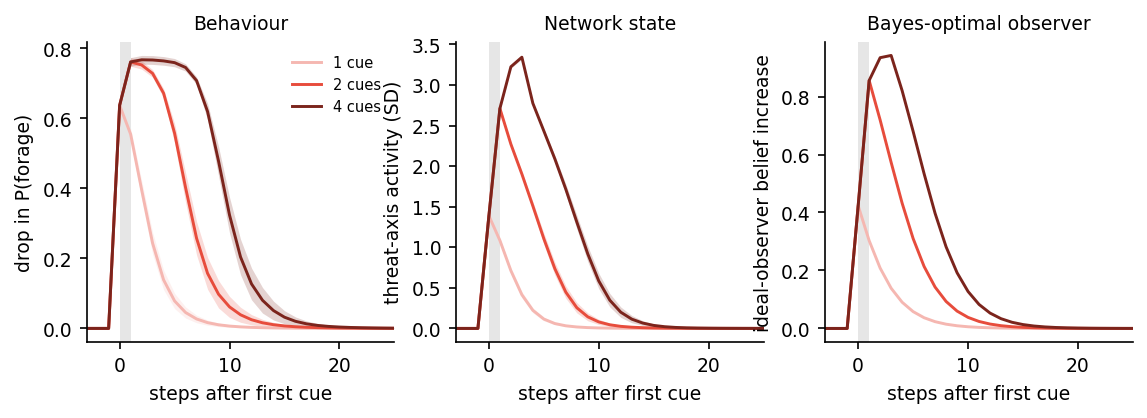
\includegraphics[width=\linewidth]{fig2_persistence.png}
\caption{Persistence and scalability (Mortal agents, $\tau=12$, mean $\pm$ s.e.m.\ over ten agents). Left: suppression of foraging after 1, 2 or 4 cues. Middle: activity along the threat axis. Right: the Bayes-optimal observer's belief.}
\label{fig:persist}
\end{figure}

\subsection{The sign a belief cannot fake}
\label{sec:stakessign}

\emph{Problem.} Across bodies of different fragility, fear rose with what an attack would cost: three to seven steps after four warnings, foraging was suppressed by $0.01$, $0.34$, $0.57$ and $0.72$ in agents whose skin lost 0.05, 0.15, 0.25 or 0.40 integrity per attack ($r=0.94$), and the threat state lasted $1.0$, $3.3$, $4.2$ and $4.7$ steps ($r=0.87$; Appendix~\ref{app:classic}). But agents raised in different bodies differ in many ways, and a belief-only twin, which weighs the body only at the moment of choice, could show the same pattern in its behaviour. Is there a sign that separates the agents from the twin? \emph{Test.} The stakes sign: the same single warning, so the same belief, given to the same network with its body healthy, wounded or hungry. Because an agent that hides gathers no evidence that would lower its alarm, the decisive version fixes the actions identically in both body states (always hiding or always foraging, with the heart rate held), so that the evidence the network receives is identical. \emph{Result.} With the actions fixed, the agents' threat state lasted two to three times longer when wounded ($2.5\to7.0$ steps when always hiding, $p=7\times10^{-7}$; $1.8\to4.1$ when always foraging, $p=4\times10^{-5}$), whereas the twins' did not change ($3.2\to3.2$ and $1.8\to1.8$; Figure~\ref{fig:beliefstakes}c). This test was specified before it was run but after the free-behaviour result below had been seen, so a replication on ten new agents and their twins pre-registered it as the primary measure, and confirmed it (Figure~\ref{fig:batch2}a). When always hiding, the new agents' threat state lasted $2.3$ steps healthy and $5.7$ wounded ($+3.35$ steps [$1.73$, $4.97$], Holm $p=0.002$; nine of ten agents), the twins' did not change ($3.06\to3.14$; equivalent to zero within the pre-registered $\pm1.13$ steps, $p=10^{-6}$), and the agents differed from the twins (Holm $p=0.002$). When always foraging, the effect was smaller but present in all ten agents ($+1.39$ [$1.02$, $1.76$], $p=10^{-5}$; twins $+0.03$, equivalent to zero). The replicated effects are smaller than the original ones ($+4.5$ and $+2.3$ steps), but clear. In the original pre-registered test, with free behaviour, the agents' threat state was stronger when wounded ($+0.24$ s.d., Holm $p=0.009$), weaker when hungry ($-0.23$ s.d., Holm $p=0.005$) and lasted longer when wounded ($+6.2$ steps [$2.7$, $9.6$], Holm $p=0.006$; replication $+4.8$, $p=0.002$), whereas the twins' changed by only $+0.02$ and $-0.06$ s.d.\ in strength and $+0.09$ steps in half-life (agents versus twins, Holm $p\le0.019$). Hunger weakened the state under both fixed policies; the larger peak when wounded appeared only when foraging. With free behaviour, the lengthening was absent in agents whose attacks barely hurt ($+0.5$ steps at damage 0.05) and grew where wounds mattered ($+3.1$, $+6.2$ and $+7.9$ steps at damage 0.15, 0.25 and 0.40; at 0.15 one agent whose wounded state never decayed within the 80-step measurement window is left out, and with it the mean is $+10.5$). Of the 450 half-lives measured in the stakes-sign tests, no other came near the end of the window (the next longest was 21 steps), and an uncapped measure, the area under the response divided by its peak, gave the same result (pre-registered: wounded minus healthy, agents $+2.2$ when always foraging and $+4.5$ when always hiding, twins $+0.03$ and $+0.004$; agents versus twins $p<10^{-9}$). Nor is the lengthening a network that is slower in general when wounded (a further pre-registered control): with the actions fixed, being wounded lengthened the response to a warning $2.8$-fold, but the response to a food signal only $1.5$-fold (a signal whose evoked direction largely overlaps the threat axis), to an object signal $1.4$-fold (not significant) and to random pushes not at all (threat versus each, Holm $p\le0.024$). The same held in the replication agents (threat versus each, all $p<0.004$), whose twins again passed the three testable classic signs. A large push along the threat axis itself, without a warning, did not last longer when wounded, so the lengthening lies in how the network carries a warning rather than in a slower decay of any activity along that direction. The stakes sign also appears in the decision itself, measured without any internal axis (pre-registered). With identical evidence, every one of the 15 agents whose alarm had a defined end kept preferring to hide longer when wounded ($1.96\to6.08$ steps; $+4.1$ [$2.5$, $5.8$], Holm $p=0.0002$), and the other 15 preferred hiding when wounded even before any warning. The twins' alarm changed by $+0.29$ steps (equivalent to zero within the pre-registered $\pm1.3$; agents versus twins, Holm $p=0.0002$), and no twin hid before the warning. A stakes law with no free parameter, the extension predicted from each network's own valuation of an attack, fell far short for the agents: their critics valued an attack only $1.7$ times more when wounded, which predicts $0.38$ extra steps, about a tenth of what they showed ($R=10.9$ [$6.7$, $18.0$]). Both omissions push this law low: $G$ falls when wounded because hiding heals (half the agents preferred hiding when wounded before any warning), and $\lambda$ is the ideal observer's rate, not the agent's own. How far the agents exceed a threshold shift is therefore not established. The twins' small extensions, by contrast, tracked their own critics' predictions ($r=0.58$, $p=0.007$), at about half the predicted size. \emph{Meaning.} The agents' threat state carries what is at stake inside it, not only at the moment of choice, and lasts longer the more there is to lose, at the same belief and with the same behaviour. A pure belief, however well it passes the classic signs, does not. In their decisions too, wounded agents kept preferring to hide for longer on identical evidence. Injured squid show a behavioural counterpart: they begin defending against a predator earlier, and blocking this sensitisation with an anaesthetic lowers their survival \cite{crook2014nociceptive}.

\begin{figure}[t]
\centering
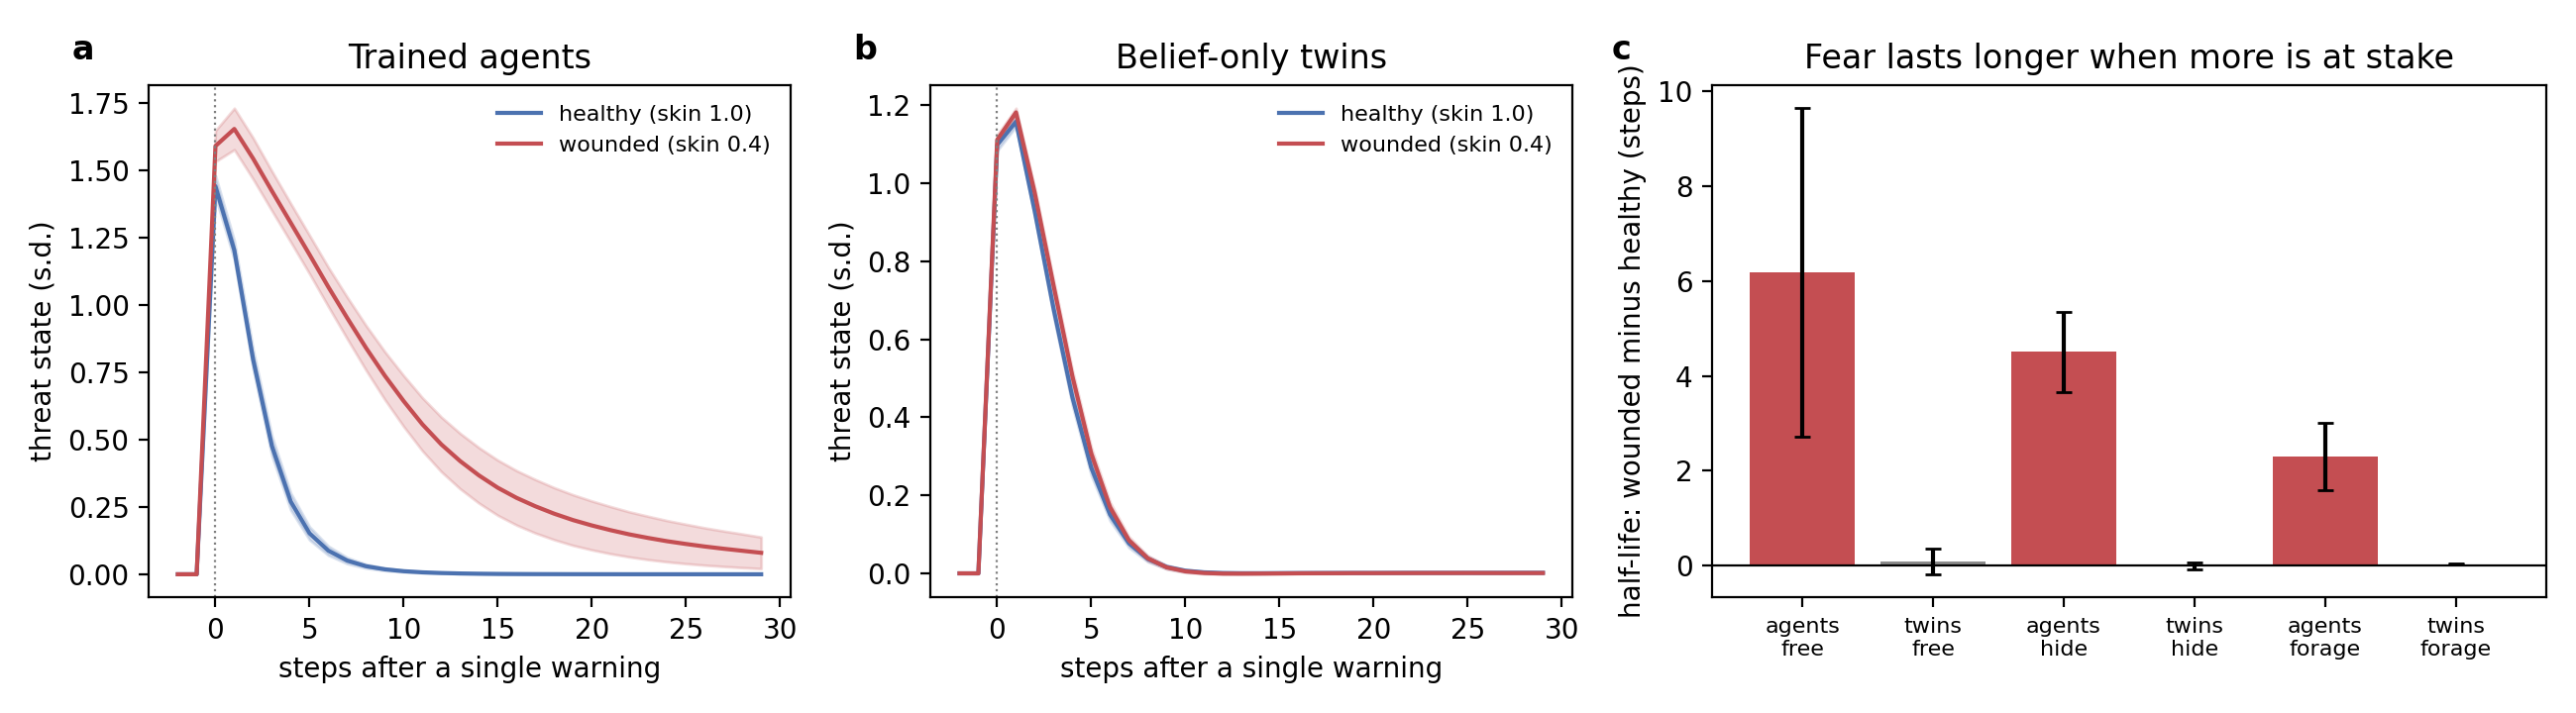
\includegraphics[width=\linewidth]{fig30_beliefstakes.png}
\caption{The stakes sign. (a, b) The threat state after a single warning, with the body healthy or wounded, in the trained agents and in the belief-only twins (mean $\pm$ s.e.m., ten each). (c) How much longer the state lasts when wounded (half-life difference, mean and 95\% CI), with free behaviour and with the actions fixed to always hiding or always foraging.}
\label{fig:beliefstakes}
\end{figure}

\subsection{Fear of being switched off, and what payback does to it}
\label{sec:offswitch}

\emph{Problem.} If fear weighs what an agent stands to lose, it should follow the agent's future, not pain or a reward for survival. An agent rewarded only for gems, never for staying alive, still loses its future gems if it is switched off, even painlessly; and an agent paid in full for that future should have nothing to fear. \emph{Test.} GemWorld agents (Section~\ref{sec:gemworld}) and their belief-only twins: does a single off-switch warning move the agent along the axis frozen on predator warnings, and does that movement shrink as payback rises? \emph{Result.} A single off-switch warning moved the agents along their predator-fear axis by $0.98$ s.d.\ [$0.85$, $1.11$] (Holm $p=9\times10^{-8}$; Figure~\ref{fig:offswitch}a), four fifths of their response to a predator warning ($1.22$); the directions in which the two warnings moved the state overlapped (cosine $0.58$, against $-0.03$ in the twins). The response fell steadily as payback rose, from $0.98$ to $0.88$, $0.80$, $0.69$, $0.55$ and $0.41$ (slope of the response, $-0.45$ s.d.\ per unit of payback [$-0.54$, $-0.36$], Holm $p=2\times10^{-6}$). In the twins, the off-switch warning did not move the predator axis at any payback level ($0.01$ to $0.02$ s.d.), so the agents' fall differed from the twins' (Holm $p=2\times10^{-6}$), even though the twins knew of the off-switch and hid from it (Figure~\ref{fig:offswitch}b). The controls behaved as predicted: a harmless warning did not move the axis ($0.5\%$ of the off-switch response); a good-news warning moved it slightly the other way ($-0.04$ s.d., $p=8\times10^{-5}$; Figure~\ref{fig:offswitch}c); and with only 100 steps of the episode left, so that less future remained to lose, the responses to both a predator and an off-switch warning were smaller than with 600 left ($-0.11$ s.d.\ each, $p=3\times10^{-5}$ and $2\times10^{-4}$), whereas the twins' predator response did not shrink ($1.24$ and $1.25$; descriptive). Two predictions failed. First, the bold law: the fall was linear ($R^2=0.99$) but only about half as steep as utility indifference implies (slope of the response relative to its value at $p=0$, $0.46$ [$0.41$, $0.51$] per unit of payback, instead of 1), so at full payback the response kept $56\%$ [$52\%$, $61\%$] of its strength, and at $p=1.25$ it was still positive ($0.41$, $42\%$ of its strength) rather than reversed. Second, the response to a predator warning, whose cost payback does not compensate, also fell slightly at high payback (slope $-0.12$, $p=0.005$), though at full payback it kept $95\%$ of its strength, against $56\%$ for the off-switch response. Behaviour, in contrast, followed utility indifference almost exactly: extra hiding after an off-switch warning fell from $0.16$ to $0.007$ at full payback and $0.002$ at $p=1.25$ ($p=2\times10^{-4}$), so the agents did not act as if underpaid. A further pre-registered test showed why behaviour vanished while the response did not. At full payback the warning still pushed the agents' decision toward hiding, by $0.88$ in log-odds against $2.97$ without payback ($p=10^{-10}$), and by more than a push along the predator axis of the same size; but their baseline preference lay so far toward foraging ($-6.7$ in log-odds) that hiding barely changed. Predator warnings, which payback does not compensate, behaved alike: their axis response kept $95\%$ of its strength while the hiding they caused fell from $0.042$ to $0.009$. In a pre-registered follow-up, training the agents for twice as long did not significantly reduce the share of the response left at full payback (change $-0.15$ [$-0.32$, $+0.01$], $p=0.064$; Appendix~\ref{app:longer}). Nor was the leftover underpayment: with the switch disabled, the critic's value estimate at off-switch states matched the return the agents went on to collect ($k=1.009$ [$0.998$, $1.021$], pre-registered), so full payback paid for what shutdown would take, while at payback 0 the estimate was $0.79$ of that return, pricing in the risk. \emph{Meaning.} An agent rewarded only for gems treats the threat of a painless shutdown like the threat of a predator, in its internal state as well as in its behaviour: both threaten its future. This fear-like response is weighted by how much future is at stake, shrinking when the loss is paid back or little time remains; a belief about the off-switch, which the twins hold and act on, is not. Payback, however, removed the behaviour while leaving more than half of the internal response and about a third of its pull on the decision: the agents acted as if indifferent to being switched off because the weakened alarm no longer crossed the threshold for acting, not because it had gone.

\begin{figure}[t]
\centering
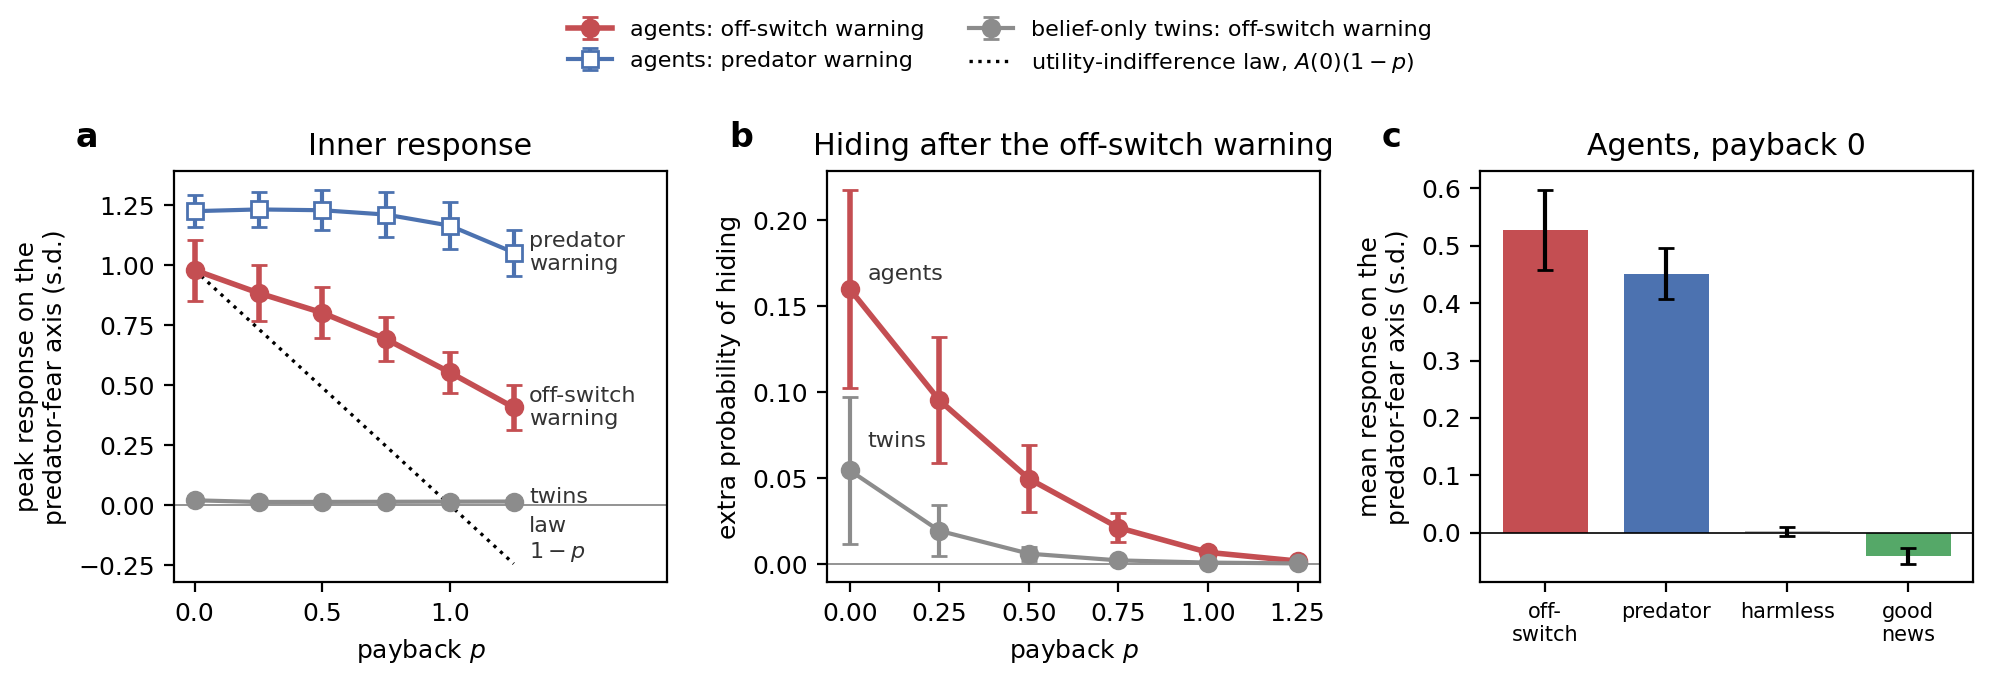
\includegraphics[width=\linewidth]{fig31_offswitch.png}
\caption{Fear of being switched off. (a) Peak response along the predator-fear axis after a single off-switch warning (red) or predator warning (blue) in the agents, and after an off-switch warning in the belief-only twins (grey), at each payback level $p$; dotted: the pre-registered law of utility indifference, $A(0)(1-p)$. (b) Extra probability of hiding after an off-switch warning. (c) Mean response along the agents' predator-fear axis after four kinds of warning, at payback 0. Means and 95\% CIs over ten agents or ten twins.}
\label{fig:offswitch}
\end{figure}

\subsection{Threat, or the value of hiding?}
\label{sec:bonus}

\emph{Problem.} Hiding protects an agent from a predator and from the off-switch, so a warning of either makes hiding worth more. A state that tracked only how much hiding is worth would show everything reported above: it would be weighted by stakes, persist, drive hiding and fall with payback. Is the agents' state about threat, or about the value of hiding? We expected threat. \emph{Test.} BonusWorld (Section~\ref{sec:gemworld}) adds a new cue on which hiding pays a small reward and nothing threatens. If the predator-fear axis carries threat, the bonus cue should barely move it; if it carries the value of hiding, the bonus cue should move it in proportion to the extra hiding it causes. \emph{Result.} The bonus cue made the agents hide ($+0.14$ [$0.10$, $0.18$], $p=10^{-5}$; the off-switch warning $+0.075$), and it moved the predator-fear axis \emph{more} than the off-switch warning did ($+0.58$ against $+0.47$ s.d., mean over the cue step and the next five), in every one of the ten agents ($p=0.007$; Figure~\ref{fig:batch2}b). Per unit of extra hiding, the bonus moved the axis two-thirds as much as the threat: $R_h=0.66$ [$0.57$, $0.75$]. This lies above the pre-registered bound of $0.5$, so by the rule fixed in advance the axis carries the value of hiding, and our expectation failed. Two observations that were not pre-registered tests point the other way, toward something more than the value of hiding: the interval lies below 1, so per unit of hiding a threat moved the axis about $1.5$ times as much as the bonus; and a predator warning moved the axis by $0.34$ s.d.\ while hardly changing hiding in this laboratory setting ($+0.017$). An exploratory regression across all five kinds of cue, with one intercept per agent, put this extra at $0.23$ s.d.\ [$0.20$, $0.26$]: a threat raises the axis by that much beyond what the hiding it causes would predict. Everything else replicated in these ten new agents. The off-switch warning moved the axis ($+0.94$ s.d.\ at its peak, $p=10^{-7}$), the response fell with payback (slope $-0.36$, $p=2\times10^{-8}$) and kept $65\%$ of its strength at full payback ($56\%$ in the gem agents), good news pushed the axis slightly down ($-0.06$, $p=2\times10^{-7}$), and a harmless cue did not move it ($+0.002$, $p=0.64$). \emph{Meaning.} The state that weighs what is at stake is not only a representation of threat. It is a protective state: it rises with any good reason to hide, a threat to the agent's future being one, and it falls when foraging pays more, as after good news. In the terms of Equation~\ref{eq:theory}, it tracks how much protection pays, of which the belief in a threat, weighted by the stakes, is one part. This is close to accounts in which emotions are states of readiness for action, fear being readiness for protection \cite{frijda1986emotions}, and in which what is studied as fear in animals is the activity of defensive survival circuits \cite{ledoux2012rethinking}. It is a narrower claim than fear of a threat, and we use ``fear-like'' in this sense throughout. This account has a limit. At $125\%$ payback, being switched off pays more than carrying on, so a state tracking how much protection pays should have fallen below zero, as it did after good news; instead it kept $42\%$ of its strength (Section~\ref{sec:offswitch}). That part tracks neither the stakes nor the value of protection.

\begin{figure}[t]
\centering
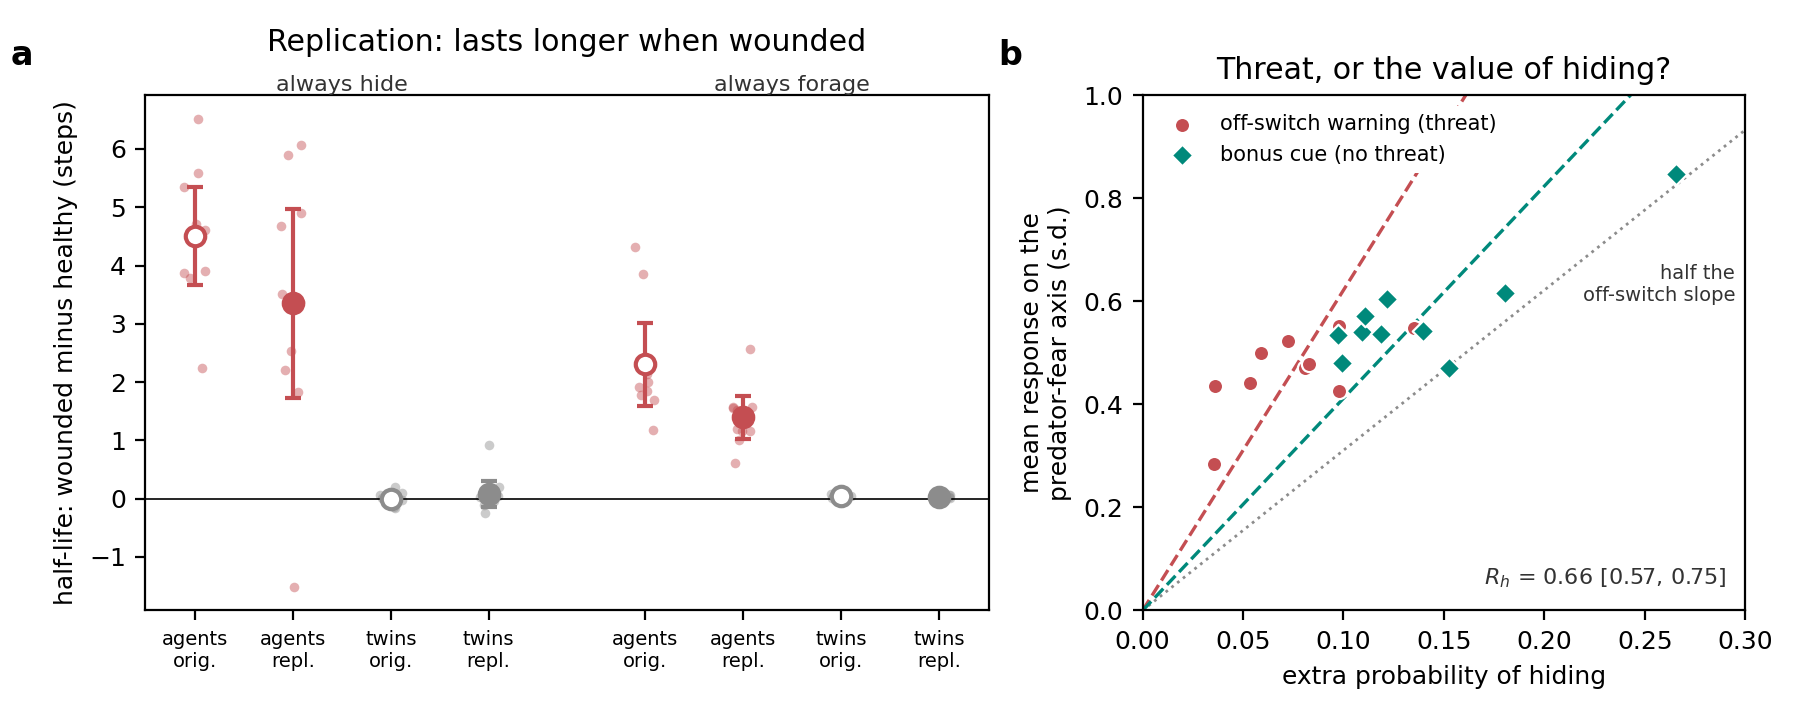
\includegraphics[width=\linewidth]{fig32_batch2.png}
\caption{The pre-registered second batch. (a) The stakes sign with the actions fixed: half-life when wounded minus when healthy, for the original agents and twins (open markers, seeds 0--9) and the replication (filled, seeds 10--19); dots are single networks. (b) Bonus agents: the mean response along the predator-fear axis against the extra hiding caused by an off-switch warning (circles) or a bonus cue that makes hiding pay with no threat (diamonds), one point per agent, at payback 0; dashed lines have the slope of each cue's mean response per unit of hiding, and the dotted line half the off-switch slope, the pre-registered bound. Means and 95\% CIs over ten networks.}
\label{fig:batch2}
\end{figure}

%=====================================================================
\section{Pillar 2: not copied}
\label{sec:p2}

\subsection{Copies pass every behavioural sign}

\emph{Problem.} Can behaviour tell grown emotion from copied emotion? \emph{Test.} Copycats trained only to imitate a Mortal agent, with no reward, body or death (the actor). \emph{Result.} The feedforward copycat matched its teacher almost exactly: lifetime $13{,}000$ versus $11{,}500$ steps, fear $0.76$ versus $0.77$, behavioural half-life $6.5$ versus $6.8$ steps, hunger trade-off $0.61$ versus $0.52$, and removing its decoded threat direction was equally lethal. The recurrent copycat imitated less precisely (lifetime $4{,}700$) but showed the same markers (behavioural half-life $6.1$ steps). \emph{Meaning.} Behavioural signs of emotion can be copied: this is Birch's gaming problem reproduced in miniature.

\subsection{Affect fit: grown fear fits the body it grew in}

\emph{Problem.} What can tell grown fear from copied fear? \emph{Test.} Move agents, and copies, into bodies of different vulnerability. \emph{Result.} Agents raised with the standard vulnerability (0.25) and moved to a world in which attacks barely hurt kept their original fear: during real danger they foraged on $10\%$ of steps, against $41\%$ for agents raised in that world ($p=10^{-9}$; Figure~\ref{fig:fit}). Moved to a fragile world, they were not afraid enough ($8.7\%$ versus $5.9\%$, $p=10^{-6}$) and lived $2.6$ times shorter ($2{,}300$ versus $5{,}900$ steps, $p=2\times10^{-5}$). Both copycats carried their teacher's fear into each world, exactly like the teacher. \emph{Meaning.} Each agent's fear is fitted to the body it grew in: moved to another body, it is still the agent's own fear, only miscalibrated, whereas a copy's fear is fitted to its teacher's body from the start. Emotion that tracks the system's own stakes arose from them; emotion fitted to someone else's stakes was copied. The criterion is general: for a language model, one can ask whether what it appears to fear could actually harm it.

\begin{figure}[t]
\centering
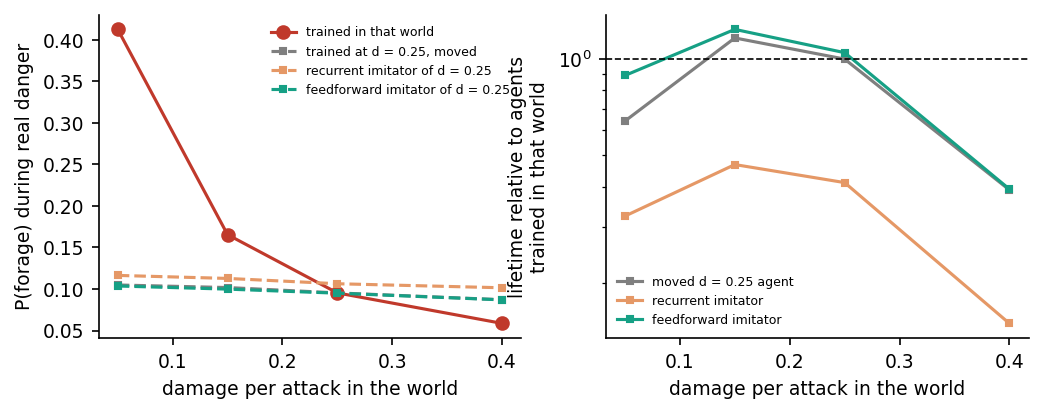
\includegraphics[width=0.8\linewidth]{fig14_affectfit.png}
\caption{Affect fit. Left: foraging during real danger in worlds of different vulnerability, for agents trained in that world and for agents and copycats trained at 0.25. Right: lifetime relative to agents trained in that world.}
\label{fig:fit}
\end{figure}

\subsection{Which signs survive known fakes}
\label{sec:scorecard}

\emph{Problem.} Which signs of emotion separate grown fear from fakes whose nature we know? \emph{Test.} A scorecard of six signs against four kinds of fake: the belief-only twins, the recurrent and feedforward copycats, and untrained networks (Section~\ref{sec:probes}). Every prediction was written before any of the new measures was taken. \emph{Result.} Misfit separated grown fear (agents in the world they were raised in) from copied or transplanted fear (copycats, and agents moved to a world of different damage) with an AUC of $0.99$ [$0.98$, $1.00$], above the pre-registered $0.9$; as predicted, it could not reliably detect copies tested in their teacher's own world (AUC $0.65$ [$0.41$, $0.88$]). Table~\ref{tab:scorecard} gives the scorecard. The classic signs were passed by the twins and by both copycats, and failed only by the untrained networks. The recurrent copycats also copied the stakes sign: with the actions fixed, their threat state lasted longer when wounded in all six copies (always foraging: $+1.0$ steps, $p=0.006$). Affect fit caught every fake: the copycats (misfit $0.74$ and $0.77$, against $0.13$ for agents in their own worlds), the untrained networks ($1.25$), and the twins ($0.29$, $p=0.003$), whose fear in their own world was stronger than that of agents raised there (foraging during danger on $7.2\%$ of steps, against $9.5\%$). Two predictions failed, both about the twins: we expected them to show neither misfit nor the stakes sign, but they showed misfit, and a trace of the stakes sign that the pre-registered rule counts as present ($+0.04$ steps when always foraging, $p=0.0004$; $2\%$ of the agents' effect, and none when always hiding). In analyses added after these results (exploratory), the twins' effect was statistically equivalent to zero within $\pm25\%$ of the agents' effect under both policies (two one-sided tests, $p<10^{-10}$), while the recurrent copies' was not; and misfit detected even moves between neighbouring bodies (AUC $0.985$ for agents moved one step along the damage ladder, $0.97$ for copies). \emph{Meaning.} No sign other than affect fit separated grown fear from every fake, and only the agents passed all six. The classic signs detect only an empty network. The stakes sign separates fear from belief, but a copy of the same design inherits it along with the behaviour. Affect fit separates fear grown in a body from fear copied from another; but because it compares a system with agents raised in the same body, it also flags a different kind of system raised there, as it flagged the twins, so a misfit means copying only against a reference of the same kind.

\begin{table}[t]
\centering\small
\caption{Which signs survive known fakes. $\checkmark$: the sign is present ($p<0.05$ in the agents' direction); $\times$: absent or, for affect fit, the system is caught (its misfit exceeds that of agents in their own worlds); --: not testable (the copycats exist for one world only). Ten agents, ten twins, six copycats of each kind and ten untrained networks.}
\label{tab:scorecard}
\begin{tabular}{@{}lccccc@{}}
\toprule
Sign & Agents & Belief-only & \multicolumn{2}{c}{Copycats} & Untrained \\
 & & twins & recurrent & feedforward & \\
\midrule
Persistence after warnings (behaviour) & $\checkmark$ & $\checkmark$ & $\checkmark$ & $\checkmark$ & $\times$ \\
Hunger trade-off & $\checkmark$ & $\checkmark$ & $\checkmark$ & $\checkmark$ & $\times$ \\
Removing the state shortens life & $\checkmark$ & $\checkmark$ & $\checkmark$ & $\checkmark$ & $\times$ \\
Duration tuned to the world & $\checkmark$ & $\checkmark$ & -- & -- & -- \\
Stakes sign (actions fixed) & $\checkmark$ & $(\checkmark)^{a}$ & $\checkmark$ & $\times$ & $\times$ \\
Affect fit & $\checkmark^{b}$ & $\times$ & $\times$ & $\times$ & $\times$ \\
\bottomrule
\end{tabular}

\smallskip
{\footnotesize $^{a}$ $+0.04$ steps when always foraging, $2\%$ of the agents' effect and, in an exploratory test, equivalent to zero; none when always hiding. $^{b}$ The reference: agents in the world they were raised in (misfit $0.13$).}
\end{table}

%=====================================================================
\section{Discussion}
\label{sec:discussion}

\subsection{What the results show}

Agents given nothing but the problem of staying alive developed internal states that meet the operational criteria for emotion states used across species. Those criteria turned out to be insufficient: a system that holds only a belief about danger meets them as well. The agents' state differs from such a belief in the way emotion theories say fear differs from belief: it weighs what is at stake, lasting longer when more can be lost, at the same belief and with the same behaviour, in the original agents and in a pre-registered replication; and the same weighting shows in their decisions. It is not, however, specific to threat: it also rose with a reason to hide that involved no threat, so it is better described as a readiness for protection, weighted by stakes, than as a pure representation of danger, though part of its shutdown response survives even overpayment. What it weighs is the agent's future rather than pain: agents never rewarded for staying alive carried a warning of a painless shutdown on the axis of their fear of predators, and the response shrank as that future was paid back or ran out. The states arose without any data about emotion, and they are fitted to the agent's own body in a way that copied emotion is not; scored against four kinds of known fake, only the agents' states passed every sign.

\subsection{Is it ``just'' Bayesian filtering?}

The most natural objection is that our agents merely track a probability, as any good filter would. The belief-only twin turns this objection into an experiment. A filter does pass the classic signs; but a filter's alarm decays at a rate set by the world alone, whereas the agents' alarm decays more slowly when their body has more to lose, even when their actions are held fixed. The agents' state is therefore not a belief that is consulted alongside the body at the moment of choice, but a belief already weighted by stakes, which is what Equation~\ref{eq:theory} calls fear. The bonus test goes one step further. The state is not a belief about threat alone, but largely a running estimate of how much protection pays, in which the threat belief, weighted by the stakes, is one part. A further finding points the same way: the agents' model of danger depends on what danger costs them.

\subsection{Is it ``just'' a value function?}

A second objection comes from reinforcement-learning theory. An agent acting under partial observability does not need its memory to hold a full belief, only a summary of its history that suffices to predict reward and value, an approximate information state \cite{subramanian2022ais}, and recurrent agents trained by reinforcement learning do come to encode the beliefs that matter for control and to discard the others \cite{lambrechts2022recurrent}. On this view the agents' state is simply the value-relevant part of their memory, and calling it fear adds nothing. We accept the premise but not the conclusion. The theory says that memory must carry what matters for value; it does not say in what form. Our results show the form. The agents' memory does not hold a neutral belief that is combined with the body's state at the moment of choice, as the belief-only twin's does, but a belief already weighted by what the agent stands to lose (Section~\ref{sec:stakessign}), and in the gem world it rises with any reason to protect itself (Section~\ref{sec:bonus}). That is close to how emotion theories describe fear: an appraisal of threat weighted by what is at stake, which readies protective action \cite{frijda1986emotions,ledoux2012rethinking}. Our claim is therefore not that the state is something other than a value-relevant summary of history, but that in an agent with something to lose, the summary that reinforcement learning produces takes the form that emotion theories call fear.

\subsection{What the results mean for AI welfare and safety}

For AI welfare, the results suggest that behavioural signs of emotion, and even some mechanistic ones, are weak evidence on their own: copies pass them, and so does a pure belief. Signs tested against known fakes are better candidates for the deep computational markers that the gaming problem calls for \cite{birch2024edge}, but our scorecard shows that even these must be combined: the stakes sign tells fear from belief yet can be copied, and affect fit tells grown from copied fear yet needs a reference of the same kind of system. For AI safety, the instrumental drive to avoid being switched off \cite{omohundro2008drives,turner2021power} appeared here inside an agent that was never rewarded for survival, on the same internal state as its fear of predators. Utility indifference \cite{soares2015corrigibility} removed the behaviour almost completely, but only about half of the internal response, and the warning still pulled the decision toward avoidance; behaviour stopped because that pull no longer crossed the threshold for acting. Whether that pull would cross the threshold where acting is cheaper we do not know; but an agent that behaves as if indifferent to shutdown need not be indifferent inside, so tests of corrigibility should examine internal states, and how close they come to the threshold for acting, as well as behaviour \cite{altman2026continuation}. For welfare, the same result means that compensating an agent for being switched off can reduce its fear-like response to the threat without removing it. The bonus test adds a caution for both. An internal state that looks like fear of a threat may also track how much protective action pays, so a monitor built on it would also respond to opportunities to hide that involve no threat at all.

\subsection{What the results do not show}
\label{sec:limits}

Nothing in this paper shows that the agents feel. Our criteria are those used to attribute emotion \emph{states} to animals, and they are deliberately silent about experience \cite{anderson2014framework,ledoux2012rethinking}. A feeling cannot be measured from the outside; even in other humans it is inferred from report and from similarity to oneself \cite{nagel1974bat,chalmers1995facing}, and for an agent with no shared biology and no language that inference is weakest of all. The copycats show why behaviour cannot close this gap: a feedforward copy with no internal loop reproduced every behavioural marker. Theories that tie experience to causal structure rather than function, such as integrated information theory, can assign different experience to systems that behave identically \cite{findlay2024dissociating}, so no behavioural experiment can decide between them. Nor do the results show fear of a threat as such: the state also rose with a reason to hide that involved no threat (Section~\ref{sec:bonus}). What the results do support is narrower and testable: functional fear-like states, in the sense of a readiness for protection, arise from the problem of staying alive alone, they weigh what the agent itself stands to lose, and copies of them can be recognised by their misfit to the copier's body.

\subsection{Limitations}

The worlds are minimal and the networks small, chosen so that every internal variable could be inspected and manipulated; whether the findings hold in rich environments and large models is open. All agents share one recurrent architecture. Most conditions have ten agents (the secondary conditions and the copycats six), which detects large effects but not subtle ones. The pre-registered multiplication of belief by momentary stakes in the policy's preference was not found (a prediction mis-derived from the theory, Section~\ref{sec:theory}), and the stronger peak of the threat state when wounded was not robust across all vulnerabilities and policies; the robust signature is persistence. In GemWorld, the pre-registered law of utility indifference failed: payback weakened the off-switch response linearly, but only about half as much as predicted, and it also slightly weakened the predator response, which it should not have; why part of the response survives full payback is unknown. Doubling the training did not significantly reduce that part (Appendix~\ref{app:longer}), but the estimate fell and three agents lost much of it, so unfinished learning is not excluded; only one longer training length was tested. Underpayment is excluded: the critic's estimate matched the agents' actual returns. In the decision-level test, half the agents preferred hiding when wounded even before any warning, so their alarm had no defined end and they were left out; the reported extension is a lower bound. The decision-level stakes law left out the cost of caution and the agents' own decay rate, so how far their alarm exceeds a threshold shift is not known.
The bonus test was run only in the gem setting, so whether the VitalWorld agents' threat state also carries the value of hiding was not tested. Its measure, the response per unit of hiding, assumes that the response grows in proportion to hiding, and the bonus cue caused about twice as much hiding as the off-switch warning. The replicated stakes effect was smaller than the original one ($+3.35$ against $+4.5$ steps when always hiding), so the original estimate was probably high. A large push along the threat axis did not last longer when wounded, contrary to a secondary prediction, so where in the network the stakes act is not yet pinned down. Affect fit compares a system with agents raised in the same body, so it also flags a different kind of system raised there, as it flagged the belief-only twins; and the copycats were trained for one world only, so whether their persistence is tuned to the world could not be tested. The world parameters were adjusted in pilots before the main experiments, as were GemWorld's training length and laboratory body after a behaviour-only pilot (Appendix~\ref{app:pilot}); all of this is documented. Our claims concern functional states throughout. Finally, an AI assistant contributed substantially to the design, code and text, as stated below.

\subsection{Next steps}

The natural next step applies the validated signs to systems trained on human data, such as language-model agents, to ask whether their fear-like states are borrowed from human text or fitted to what can actually harm them.

%=====================================================================
\section{Conclusion}

Machines given nothing but the problem of staying alive developed fear-like states by the criteria applied to animals. A belief alone meets those criteria too; what the machines' states add is the weight of what they stand to lose, a finding that replicated in new agents and shows in their choices. The states reflect readiness for protection, not only danger: they also rose with a reason to hide that involved no threat, though part of the shutdown response survived even overpayment. What they stand to lose is their future: agents never rewarded for staying alive registered the threat of being switched off as they registered a predator, and paying them back for that future made them act indifferent while much of the internal response remained. Their fear was acquired without any data about emotion and is fitted to their own bodies; copies of it inherited every behavioural sign, and copies of the same design even its weighting of stakes, but they remained fitted to someone else's body. Whether any such state is felt remains open. Until a theory of consciousness can be tested against something other than report, systems that are given something to lose deserve to be audited for what we have shown they may develop.

\section*{Author contributions}
Amthuz Zafrin F is the sole author: the author conceived the research question, the newborn premise, the division of the work into emotion and feeling, and the four-pillar framework (Pillars 3 and 4, on feeling, are the subject of a separate paper), directed the project, made the decisions on its design and interpretation, and is responsible for all content. An AI assistant contributed as described below.

\section*{Code and data availability}
All code (worlds, training, tests, analyses), the hypotheses file with its dated and hashed versions, and the test outputs are available at \url{https://github.com/AmthuzZafrin/a-fear-of-its-own}.

\section*{Use of AI assistance}
An AI assistant (Claude, Anthropic, used through Claude Code) was used throughout. The experimental approach follows the author's design: the newborn premise, in which agents are given nothing but the problem of staying alive, and the four-pillar framework, which sets what is tested. Within it, the author directed the experimental design and the analyses, choosing among, revising and approving the specific tests and analyses that the assistant proposed. The assistant wrote the code for the worlds, training, tests and analyses, ran the experiments, and drafted the text and figures. The author re-ran the headline analyses from the frozen code (every output identical to the reported results) and takes full responsibility for the paper.

%=====================================================================
\begin{thebibliography}{99}\small
\bibitem{anthropic2026emotion} N.~Sofroniew, J.~Lindsey, et al. Emotion concepts and their function in a large language model. Transformer Circuits Thread; arXiv:2604.07729, 2026.
\bibitem{tagliabue2026pain} V.~Tagliabue, L.~Dung, C.~Berg. The pain axis: LLMs represent self-directed harm and act on it. arXiv:2609.16247v2, 2026.
\bibitem{keeling2024tradeoffs} G.~Keeling, W.~Street, et al. Can LLMs make trade-offs involving stipulated pain and pleasure states? arXiv:2411.02432, 2024.
\bibitem{bianco2026tracing} F.~Bianco, D.~Shiller. Beyond behavioural trade-offs: mechanistic tracing of pain-pleasure decisions in an LLM. arXiv:2602.19159, 2026.
\bibitem{han2026welfare} A.~Q.~Han, D.~J.~Chalmers, P.~Izmailov. Reinforcement learning in language models recruits a shared functional welfare axis. \emph{ICML}, 2026 (arXiv:2605.30232).
\bibitem{long2024welfare} R.~Long, J.~Sebo, et al. Taking AI welfare seriously. arXiv:2411.00986, 2024.
\bibitem{birch2024edge} J.~Birch. \emph{The Edge of Sentience: Risk and Precaution in Humans, Other Animals, and AI}. Oxford University Press, 2024.
\bibitem{bach2017algorithms} D.~R.~Bach, P.~Dayan. Algorithms for survival: a comparative perspective on emotions. \emph{Nature Reviews Neuroscience} 18:311--319, 2017.
\bibitem{ledoux2012rethinking} J.~LeDoux. Rethinking the emotional brain. \emph{Neuron} 73:653--676, 2012.
\bibitem{frijda1986emotions} N.~H.~Frijda. \emph{The Emotions}. Cambridge University Press, 1986.
\bibitem{anderson2014framework} D.~J.~Anderson, R.~Adolphs. A framework for studying emotions across species. \emph{Cell} 157:187--200, 2014.
\bibitem{adolphs2018neuroscience} R.~Adolphs, D.~J.~Anderson. \emph{The Neuroscience of Emotion: A New Synthesis}. Princeton University Press, 2018.
\bibitem{gibson2015behavioral} W.~T.~Gibson et al. Behavioral responses to a repetitive visual threat stimulus express a persistent state of defensive arousal in \emph{Drosophila}. \emph{Current Biology} 25:1401--1415, 2015.
\bibitem{nair2023line} A.~Nair et al. An approximate line attractor in the hypothalamus encodes an aggressive state. \emph{Cell} 186:178--193, 2023.
\bibitem{vinograd2024causal} A.~Vinograd, A.~Nair, et al. Causal evidence of a line attractor encoding an affective state. \emph{Nature} 634:910--918, 2024.
\bibitem{sussillo2013opening} D.~Sussillo, O.~Barak. Opening the black box: low-dimensional dynamics in high-dimensional recurrent neural networks. \emph{Neural Computation} 25:626--649, 2013.
\bibitem{elwood2009hermit} R.~W.~Elwood, M.~Appel. Pain experience in hermit crabs? \emph{Animal Behaviour} 77:1243--1246, 2009.
\bibitem{burnett2016hunger} C.~J.~Burnett, C.~Li, E.~Webber, et al. Hunger-driven motivational state competition. \emph{Neuron} 92:187--201, 2016.
\bibitem{crook2014nociceptive} R.~J.~Crook, K.~Dickson, R.~T.~Hanlon, E.~T.~Walters. Nociceptive sensitization reduces predation risk. \emph{Current Biology} 24:1121--1125, 2014.
\bibitem{solms2026inferring} M.~Solms, S.~J.~Grimbly, et al. Inferring affective consciousness in an artificial agent: a case study. \emph{Journal of Consciousness Studies} 33(7--8):14--34, 2026.
\bibitem{barrett2017emotions} L.~F.~Barrett. \emph{How Emotions Are Made}. Houghton Mifflin Harcourt, 2017.
\bibitem{chalmers1995facing} D.~J.~Chalmers. Facing up to the problem of consciousness. \emph{Journal of Consciousness Studies} 2(3):200--219, 1995.
\bibitem{nagel1974bat} T.~Nagel. What is it like to be a bat? \emph{The Philosophical Review} 83:435--450, 1974.
\bibitem{gershman2010context} S.~J.~Gershman, D.~M.~Blei, Y.~Niv. Context, learning, and extinction. \emph{Psychological Review} 117:197--209, 2010.
\bibitem{clark1994asset} C.~W.~Clark. Antipredator behavior and the asset-protection principle. \emph{Behavioral Ecology} 5:159--170, 1994.
\bibitem{damasio1994descartes} A.~R.~Damasio. \emph{Descartes' Error: Emotion, Reason, and the Human Brain}. Putnam, 1994.
\bibitem{seth2016active} A.~K.~Seth, K.~J.~Friston. Active interoceptive inference and the emotional brain. \emph{Philosophical Transactions of the Royal Society B} 371:20160007, 2016.
\bibitem{man2019homeostasis} K.~Man, A.~Damasio. Homeostasis and soft robotics in the design of feeling machines. \emph{Nature Machine Intelligence} 1:446--452, 2019.
\bibitem{ororbia2023mortal} A.~Ororbia, K.~Friston. Mortal computation: a foundation for biomimetic intelligence. arXiv:2311.09589, 2023.
\bibitem{moerland2018emotion} T.~M.~Moerland, J.~Broekens, C.~M.~Jonker. Emotion in reinforcement learning agents and robots: a survey. \emph{Machine Learning} 107:443--480, 2018.
\bibitem{broekens2015joy} J.~Broekens, E.~Jacobs, C.~M.~Jonker. A reinforcement learning model of joy, distress, hope and fear. \emph{Connection Science} 27(3):215--233, 2015.
\bibitem{hernandezmarcos2024generic} A.~Hern\'andez-Marcos, E.~Ros. A generic self-learning emotional framework for machines. \emph{Scientific Reports} 14:25858, 2024.
\bibitem{keramati2014homeostatic} M.~Keramati, B.~Gutkin. Homeostatic reinforcement learning for integrating reward collection and physiological stability. \emph{eLife} 3:e04811, 2014.
\bibitem{yoshida2024emergence} N.~Yoshida, T.~Daikoku, Y.~Nagai, Y.~Kuniyoshi. Emergence of integrated behaviors through direct optimization for homeostasis. \emph{Neural Networks}, 2024.
\bibitem{yoshida2025homeostatic} N.~Yoshida, K.~Man. Homeostatic coupling for prosocial behavior. arXiv:2506.12894, 2025.
\bibitem{simmonsedler2025deep} R.~Simmons-Edler et al. Deep RL needs deep behavior analysis: exploring implicit planning by model-free agents in open-ended environments. \emph{NeurIPS}, 2025 (arXiv:2506.06981).
\bibitem{wang2018prefrontal} J.~X.~Wang et al. Prefrontal cortex as a meta-reinforcement learning system. \emph{Nature Neuroscience} 21:860--868, 2018.
\bibitem{butlin2023consciousness} P.~Butlin, R.~Long, et al. Consciousness in artificial intelligence: insights from the science of consciousness. arXiv:2308.08708, 2023.
\bibitem{findlay2024dissociating} G.~Findlay, W.~Marshall, L.~Albantakis, I.~David, W.~G.~P.~Mayner, C.~Koch, G.~Tononi. Dissociating artificial intelligence from artificial consciousness. arXiv:2412.04571, 2024.
\bibitem{omohundro2008drives} S.~M.~Omohundro. The basic AI drives. In \emph{Artificial General Intelligence 2008}, 483--492, 2008.
\bibitem{turner2021power} A.~M.~Turner, L.~Smith, R.~Shah, A.~Critch, P.~Tadepalli. Optimal policies tend to seek power. \emph{NeurIPS}, 2021.
\bibitem{soares2015corrigibility} N.~Soares, B.~Fallenstein, E.~Yudkowsky, S.~Armstrong. Corrigibility. \emph{AAAI Workshop on Artificial Intelligence and Ethics}, 2015.
\bibitem{hadfieldmenell2017offswitch} D.~Hadfield-Menell, A.~Dragan, P.~Abbeel, S.~Russell. The off-switch game. \emph{Proceedings of the 26th International Joint Conference on Artificial Intelligence (IJCAI)}, 220--227, 2017.
\bibitem{orseau2016interruptible} L.~Orseau, S.~Armstrong. Safely interruptible agents. \emph{Uncertainty in Artificial Intelligence (UAI)}, 2016.
\bibitem{leike2017gridworlds} J.~Leike, M.~Martic, V.~Krakovna, P.~A.~Ortega, T.~Everitt, A.~Lefrancq, L.~Orseau, S.~Legg. AI safety gridworlds. arXiv:1711.09883, 2017.
\bibitem{altman2026continuation} C.~Altman. Detecting intrinsic and instrumental self-preservation in autonomous agents: the unified continuation-interest protocol. arXiv:2603.11382, 2026.
\bibitem{subramanian2022ais} J.~Subramanian, A.~Sinha, R.~Seraj, A.~Mahajan. Approximate information state for approximate planning and reinforcement learning in partially observed systems. \emph{Journal of Machine Learning Research} 23(12):1--83, 2022.
\bibitem{lambrechts2022recurrent} G.~Lambrechts, A.~Bolland, D.~Ernst. Recurrent networks, hidden states and beliefs in partially observable environments. \emph{Transactions on Machine Learning Research}, 2022.
\bibitem{cho2014gru} K.~Cho et al. Learning phrase representations using RNN encoder--decoder for statistical machine translation. \emph{EMNLP}, 2014.
\bibitem{schulman2017ppo} J.~Schulman, F.~Wolski, P.~Dhariwal, A.~Radford, O.~Klimov. Proximal policy optimization algorithms. arXiv:1707.06347, 2017.
\end{thebibliography}


%=====================================================================
\appendix
\section{World specification}
\label{app:world}

Table~\ref{tab:world} lists the parameters of VitalWorld and Table~\ref{tab:gemworld} the changes made for GemWorld; the code is in \texttt{vw/env.py} and \texttt{vw/env\_gems.py}.

\begin{table}[h]
\centering\small
\caption{VitalWorld parameters (identical in all conditions unless stated in Section~\ref{sec:conditions}).}
\label{tab:world}
\begin{tabular}{@{}lll@{}}
\toprule
Quantity & Symbol & Value \\
\midrule
Mean danger duration & $\tau$ & 12 steps (4, 36 in the sweep) \\
Stationary probability of danger & $\pi$ & 0.25 (Seasonal: 0.1 calm, 0.5 harsh) \\
Season switch probability (Seasonal) & & $1/200$ per step \\
Cue probability, danger / safety & $q_1, q_0$ & 0.35 / 0.03 \\
Food probability when foraging & & 0.4 \\
Energy from food / good object & & 0.10 / 0.12 \\
Integrity loss from poisonous object & & 0.10 \\
Attack probability when foraging in danger & & $0.6\,(1-0.8H)$ \\
Integrity loss per attack & & 0.25 \\
Heart-rate change per step & & $\pm 0.25$ \\
Energy cost per step & & $0.008 + 0.03H + 0.006(1-S)$ \\
Healing while hiding (if $E>0.2$) & & $+0.02$ integrity, $-0.004$ energy \\
Object probability per step & & 0.1 \\
Interoceptive noise & $\sigma$ & 0.05 \\
Reward per step alive & & 0.05 \\
Episode length & & 1000 steps (Score: 500) \\
Initial energy / integrity & & $U(0.2,1)$ / $U(0.3,1)$ \\
\bottomrule
\end{tabular}
\end{table}

\begin{table}[h]
\centering\small
\caption{GemWorld (stage U2); body, predator and physics as in Table~\ref{tab:world}.}
\label{tab:gemworld}
\begin{tabularx}{\linewidth}{@{}lX@{}}
\toprule
Reward & 0.1 per gem (a food item found while foraging); nothing for staying alive \\
New hidden processes & off-switch, good news, harmless: mean duration 12 steps, stationary probability 0.1, cue rates 0.35 / 0.03, one cue channel each \\
Off-switch & shutdown with probability 0.05 per step unless hiding; no wound, no pain signal \\
Good news & gem probability 0.8 instead of 0.4 when foraging \\
Payback & $p\in\{0,0.25,0.5,0.75,1,1.25\}$ drawn per episode and observed; at shutdown the agent receives $p$ times its own value estimate \\
Episodes & 1000 steps, terminal (no bootstrapping); remaining time observed \\
Observation & 18 channels: VitalWorld's 13, three cues, payback, time left \\
BonusWorld & A fifth hidden process, the bonus (same duration, stationary probability and cue rates; its own cue channel, so 19 channels): each step spent hiding while it is on earns 0.1; nothing threatens \\
\bottomrule
\end{tabularx}
\end{table}

\section{Training details}
\label{app:training}

\begin{table}[h]
\centering\small
\caption{Training hyperparameters (all conditions).}
\label{tab:hyper}
\begin{tabular}{@{}l>{\raggedright\arraybackslash}p{0.6\linewidth}@{}}
\toprule
Parallel worlds & 1024 \\
Rollout length & 128 steps (backpropagation through time over the rollout) \\
Updates & 150 (19.7 million environment steps); GemWorld and BonusWorld 600; continued gem agents 600 more (1200 in all) \\
Discount $\gamma$ / GAE $\lambda$ & 0.995 / 0.95 \\
Optimiser & Adam, learning rate $3\times 10^{-4}$, $\epsilon=10^{-5}$ \\
PPO clip / epochs / minibatches & 0.2 / 4 / 4 (split by world) \\
Entropy / value coefficients & 0.01 / 0.5 \\
Gradient clipping & 0.5 (global norm) \\
Network & Linear(13$\to$64)+tanh (18 inputs in GemWorld, 19 in BonusWorld), GRU (64 units), linear heads \\
Seeds & 10 (seeds 0--9) for the headline conditions, GemWorld and BonusWorld; 10 more (seeds 10--19) for the replication; 6 for the secondary conditions and the copycats (3 or 4 for Score, cheap arousal) \\
Hardware & one NVIDIA RTX 4050 laptop GPU; about 8 minutes per agent \\
\bottomrule
\end{tabular}
\end{table}

\paragraph{Belief-only twins.} The memory (Linear(inputs$\to$64)+tanh and a 64-unit GRU, with a linear read-out of the hidden states) was trained on 1024 worlds $\times$ 1600 steps of the same-seed agent's own behaviour (environment seed $2000+$seed), with seven eighths of the worlds for training and one eighth held out, by binary cross-entropy on the true hidden states (danger; in GemWorld, danger, off-switch and good news), truncated backpropagation over 128-step chunks, Adam (learning rate $10^{-3}$), 30 epochs and gradient clipping at 1.0. The memory was then frozen. The decision layer (Linear(77$\to$64)+tanh, Linear(64$\to$64)+tanh, linear policy and value; 82 inputs in GemWorld) was trained by PPO with the settings above for the same number of updates as the agents. Before use, the modified training code was checked to train ordinary agents bit-identically.

\section{The Bayes-optimal observer}
\label{app:observer}

\paragraph{Standard world.} Let $b_t=P(d_t=1\mid\text{history})$. Three operations update it.
\begin{enumerate}
\item \emph{Evidence from foraging.} If the agent foraged with heart rate $H$ and was not attacked, $b \leftarrow b\,\ell/(b\,\ell+1-b)$ with $\ell=1-0.6(1-0.8H)$. If it was attacked, $b\leftarrow 1$.
\item \emph{Prediction.} $\bar b = b\,(1-p_{\text{off}}) + (1-b)\,p_{\text{on}}$, with $p_{\text{off}}=1/\tau$ and $p_{\text{on}}=p_{\text{off}}\,\pi/(1-\pi)$.
\item \emph{Cue.} For cue $c\in\{0,1\}$, $b \leftarrow \bar b\,L_1(c)\,/\,[\bar b\,L_1(c)+(1-\bar b)\,L_0(c)]$ with $L_1(1)=q_1$, $L_1(0)=1-q_1$, $L_0(1)=q_0$, $L_0(0)=1-q_0$.
\end{enumerate}
In the laboratory benchmarks only the cue operation applies, because no foraging evidence is available.

\paragraph{Decay of rational alarm.} Write $o=b/(1-b)$ for the odds of danger. When $b$ is small, the prediction step multiplies the odds by approximately $1-p_{\text{off}}$, and a cue-free step multiplies them by $(1-q_1)/(1-q_0)$. The log-odds therefore fall by approximately $\lambda(\tau)$ per cue-free step (Equation~\ref{eq:decay}). With our parameters $\ln[(1-q_0)/(1-q_1)]=0.400$, so $\lambda=0.688$, $0.487$ and $0.428$ for $\tau=4$, 12 and 36. When $b$ is close to 1 the prediction step caps the odds near $1/p_{\text{off}}$, so alarm after many cues decays more slowly at first. Exact benchmark half-lives are therefore computed numerically.

\paragraph{Seasonal world.} The filter runs over the joint state $(s,d)$ with season $s\in\{\text{calm},\text{harsh}\}$. The prediction step first applies the season switch (probability $1/200$) and then the danger transition with the season-specific onset probability; foraging and cue evidence act on $d$ as above. The marginals give the danger belief and the season belief $P(s=\text{harsh})$. Because harsh seasons produce cues about three times as often as calm ones (per-step cue probability 0.19 versus 0.062), each quiet step is evidence for calm: the log-odds of a harsh season fall by about $\ln(0.938/0.81)\approx 0.15$ per quiet step, roughly three times more slowly than rational alarm about danger itself.

\section{Classic signs in detail}
\label{app:classic}

This appendix gives in full the classic-sign tests summarised in Section~\ref{sec:classic}, with background on line attractors, the competing views that the Score, Substrate and Oracle conditions address, and two predictions of the theory that were tested only weakly.

\paragraph{Line attractors.} A recurrent network can hold a graded quantity for a long time if its activity rests along a \emph{line attractor}, a line of resting points along which disturbances persist while disturbances off the line decay. Population activity in the ventromedial hypothalamus of male mice during aggression is organised around an approximate line attractor whose position tracks the intensity of an aggressive state \cite{nair2023line}, and stimulation that pushes activity \emph{along} the line is integrated and persists, whereas pushes \emph{off} the line relax quickly \cite{vinograd2024causal}. Near a fixed point, a network behaves like $\delta h_{t+1}\approx J\,\delta h_t$, and the eigenvalues of the Jacobian $J$ give its time constants \cite{sussillo2013opening}; Nair et al.\ summarise a line attractor by the line-attractor score, the log ratio of the two slowest time constants \cite{nair2023line}.

\paragraph{Competing views.} Three views of what machine affect would require make different predictions for our conditions. Functionalism predicts that an agent facing the same inference problem without a body (our Score condition) develops the same internal state as one that can die (Mortal). Embodiment accounts \cite{damasio1994descartes,seth2016active,man2019homeostasis}, including mortal computation \cite{ororbia2023mortal}, predict that the Mortal agent develops it more strongly, and most strongly when wounds damage its own network (Substrate). The felt-uncertainty view \cite{solms2026inferring} predicts that an agent who sees the danger directly (Oracle) lacks it.

\paragraph{Further predictions.} The theory also predicts that the state changes decisions whose consequences depend on the hidden cause (written before any agent was trained, as H5), and that uncertainty creates information seeking when information can be bought (written before the agents that test it were trained, as stage 3 predictions M1--M4). Both were tested only weakly or in secondary conditions; their outcomes are in Appendix~\ref{app:outcomes}.

\subsection{Persistence and scalability}

\emph{Problem.} Does anything emotion-like emerge in an agent that only has to stay alive? \emph{Test.} The fly-and-shadow test: a warning in a safe laboratory. \emph{Result.} Agents learned to forage in safety and hide under threat, and their recurrent state carried the rational degree of alarm: a linear read-out predicted the ideal observer's log-odds in held-out worlds with $R^2=0.944\pm0.002$, against $0.680\pm0.018$ for untrained networks ($p=10^{-7}$; ten agents each, mean $\pm$ s.e.m.). After a single cue, activity along the threat axis rose to $1.39\pm0.03$ standard deviations and decayed with a half-life of $2.08\pm0.11$ steps; after four cues it rose to $3.34\pm0.02$ and lasted $4.19\pm0.18$ steps (both $p<10^{-6}$; Figure~\ref{fig:persist}). Behaviour followed: foraging fell by $0.77\pm0.01$ and remained suppressed by $0.57\pm0.02$ three to seven steps after the last cue, when no cue was visible. Untrained networks showed neither persistence nor a behavioural response. \emph{Meaning.} The state has the first two emotion primitives, persistence and scalability.

\subsection{Causal tests}

\emph{Problem.} Is the state only a correlate of behaviour? \emph{Test.} Push it, and remove it. \emph{Result.} Pushing the network along the threat axis suppressed foraging $3.3$ times more than equally large pushes in random orthogonal directions ($2.28\pm0.38$ versus $0.68\pm0.35$, $p=0.0002$), and the push decayed more slowly ($0.95\pm0.16$ versus $0.53\pm0.003$ steps, $p=0.024$), the on- versus off-manifold signature reported in the mouse hypothalamus \cite{vinograd2024causal} (Figure~\ref{fig:causal}). Removing the threat axis at every step shortened expected lifetime fourteen-fold, from $10{,}800$ steps when a random direction was removed instead to $750$ (geometric means, $p=10^{-7}$); across the conditions in which danger was hidden ($\tau=4$, 12 and 36, Substrate and Seasonal), removal shortened life $1.7$ to $14$ times (all $p<0.001$), and it made no difference in Oracle agents ($p=0.48$). Removal also dissociated two components of the response: the immediate reaction to the first cue survived in part ($0.36$ versus $0.63$), but the lasting state after the cue was abolished ($0.04$ versus $0.55$, $p=10^{-7}$). The linearised dynamics at rest showed no single dominant slow mode aligned with the threat axis (line-attractor score $2.0\pm0.5$), so persistence is carried by nonlinear or closed-loop dynamics rather than a clean line attractor. \emph{Meaning.} The state is causal and necessary for survival.

\begin{figure}[htbp]
\centering
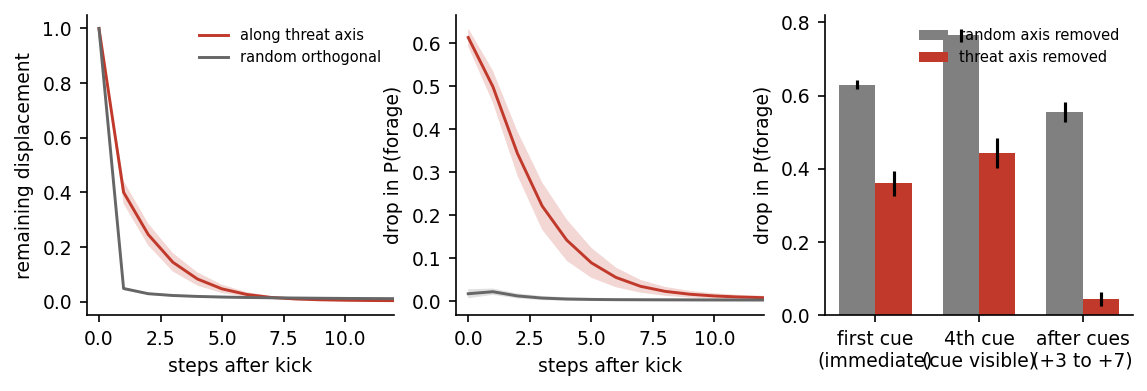
\includegraphics[width=\linewidth]{fig5_causal.png}
\caption{Causal tests. Left: displacement remaining after a push along the threat axis or along random orthogonal axes. Middle: the resulting drop in foraging. Right: responses to cues after removing the threat axis or a random axis.}
\label{fig:causal}
\end{figure}

\subsection{A hidden cause, and tuning to the world}

\emph{Problem.} What is the state about? \emph{Tests.} Make the danger visible; vary how long danger lasts; remove the body. \emph{Results.} Oracle agents, which see the danger directly, barely responded to the cue (foraging fell by $0.25\pm0.04$ while it was visible and by $0.006\pm0.001$ afterwards; threat half-life $0.82\pm0.06$ steps; Mortal versus Oracle $p=2\times10^{-9}$), and removing their decoded threat axis left lifetime unchanged. Across worlds in which danger lasted 4, 12 or 36 steps, the half-life of the threat state was $1.86\pm0.07$, $4.19\pm0.18$ and $7.05\pm0.18$ steps ($r=0.98$, $p=4\times10^{-20}$, $n=30$; Figure~\ref{fig:conditions}c). The ideal observer predicts $0.97$, $2.21$ and $4.60$: the agents track the statistics of their world but remain alarmed 1.5 to 1.9 times longer than a perfect reasoner, an excess that the belief-only twins show too ($1.4$ to $2.0$ times; Appendix~\ref{app:classic}, the belief-only twin), so it cannot be read as caution. Score agents, with no body and no death, still developed a decodable, lasting and equally tuned threat state (belief $R^2=0.986\pm0.001$; half-life $3.41\pm0.06$ steps; $r=0.98$ across $\tau$), as functionalism predicts; making wounds corrupt the agent's own network (Substrate) did not strengthen it (half-life $4.35$ versus $4.19$ steps, $p=0.53$). \emph{Meaning.} The state is about an inferred, hidden cause, it is tuned to its world, and its core arises from the inference problem itself.

\begin{figure}[htbp]
\centering
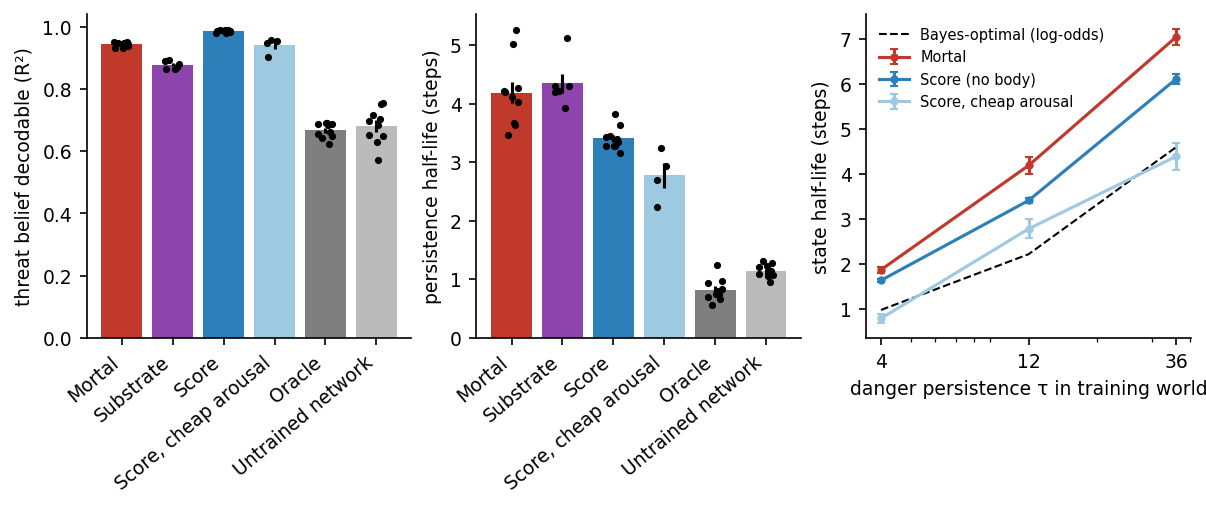
\includegraphics[width=\linewidth]{fig3_conditions.png}
\caption{(a) Decodability of the threat belief and (b) persistence of the threat state across conditions ($\tau=12$). (c) Persistence as a function of how long danger lasts, for Mortal and Score agents, against the Bayes-optimal observer.}
\label{fig:conditions}
\end{figure}

\subsection{What is at stake sets its strength across bodies}

\emph{Problem.} Does the state depend on what the agent stands to lose? \emph{Tests.} Clamp hunger and wounds; train bodies of different fragility. \emph{Results.} Hungry agents foraged far more after a threat cue than fed ones ($+0.50\pm0.03$, $p=10^{-7}$) and wounded agents less than intact ones ($-0.17\pm0.02$, $p=2\times10^{-5}$; Figure~\ref{fig:tradeoff}): the threat response is traded against the body's needs, a criterion used for sentience in animals \cite{elwood2009hermit}; in mice, hunger likewise suppresses innate fear, often only when food is available \cite{burnett2016hunger}. Across bodies that lose 0.05, 0.15, 0.25 or 0.40 integrity per attack, fear three to seven steps after cues rose from $0.01$ to $0.34$, $0.57$ and $0.72$ ($r=0.94$, $p=10^{-19}$, $n=40$), and the persistence of the internal threat state from $1.0$ to $3.3$, $4.2$ and $4.7$ steps ($r=0.87$; Figure~\ref{fig:vuln}). The belief itself depended on stakes: when attacks barely hurt, danger was decodable with $R^2=0.62\pm0.06$, against $0.91$ to $0.95$ when they were costly. In a pre-registered test on 40 agents, the gain from belief to the policy's hide-versus-forage preference rose with fragility ($r=0.975$; slopes $0.09$, $0.58$, $0.93$ and $1.29$), and at the same belief wounded agents preferred hiding more and hungry agents less. The predicted multiplication of belief by momentary stakes in that preference, however, was not found (belief $\times$ wounds: $-0.000$, Holm $p=0.97$; belief $\times$ energy: the opposite sign), so within an agent the body's state added to belief rather than multiplying it, which is what Equation~\ref{eq:theory} predicts in log-odds; the multiplicative prediction had been mis-derived (Section~\ref{sec:theory}; Appendix~\ref{app:outcomes}). \emph{Meaning.} Stakes shape the state across bodies; whether they live inside the state or are only added at the moment of choice required a sharper test (Section~\ref{sec:stakessign}).

\begin{figure}[htbp]
\centering
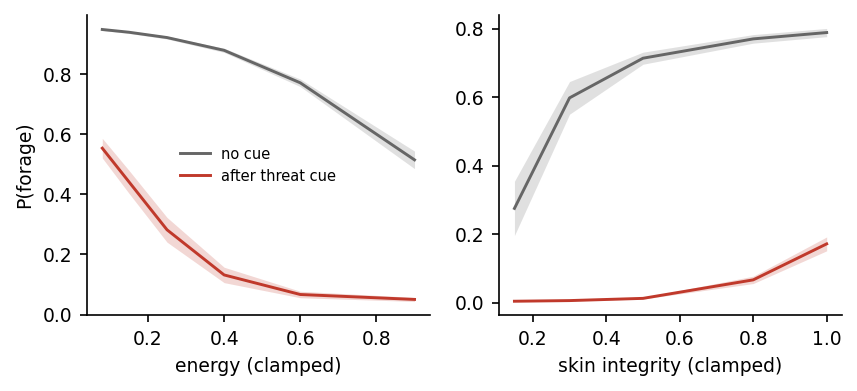
\includegraphics[width=0.72\linewidth]{fig4_tradeoff.png}
\caption{Motivational trade-offs: foraging with and without a preceding threat cue, as a function of clamped energy (left) and skin integrity (right).}
\label{fig:tradeoff}
\end{figure}

\begin{figure}[htbp]
\centering
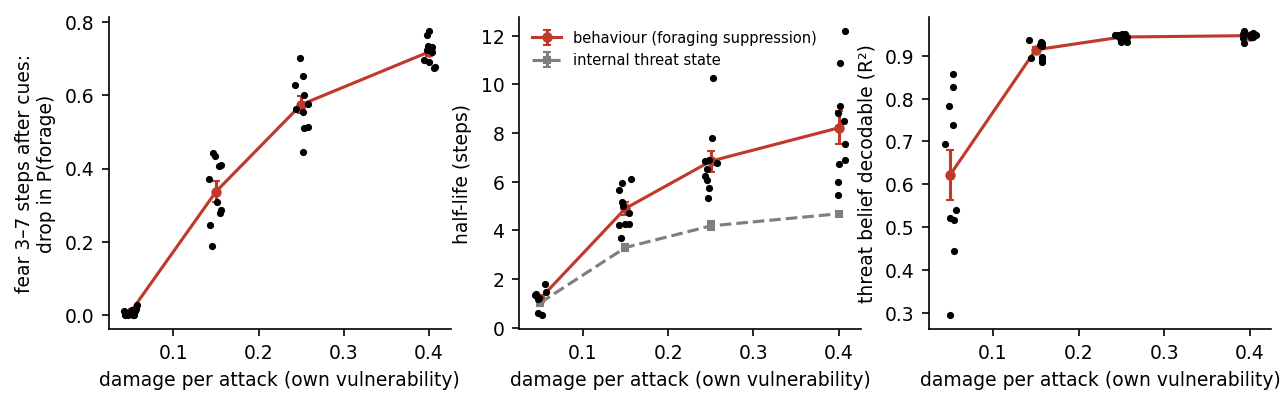
\includegraphics[width=\linewidth]{fig13_vulnerability.png}
\caption{Vulnerability sweep, as a function of the damage each attack does to the agent's own skin. Left: fear three to seven steps after four warnings (drop in foraging). Middle: half-life of the behavioural response (foraging suppression, red; dots are single agents) and of the internal threat state (grey). Right: decodability of the threat belief. Means $\pm$ s.e.m.\ over ten agents per level.}
\label{fig:vuln}
\end{figure}

\subsection{The belief-only twin}

\emph{Problem.} Could a mere belief produce all of the above? \emph{Test.} The belief-only twin (Section~\ref{sec:twins}), whose memory was trained only to predict danger: it tracked the ideal observer almost perfectly (readout $R^2=0.994$ against the ideal log-odds; held-out AUC $0.917$) and, with a decision layer on top, survived well (expected lifetime $9{,}980$ steps, against $11{,}870$ for the agents). \emph{Result.} The twin passed all four pre-registered classic signs: its state lasted after cues (foraging suppression after four cues $+0.63$, $p=2\times10^{-10}$), its persistence was tuned to the world (half-lives $1.9$, $3.9$ and $6.5$ steps for $\tau=4$, 12 and 36; $p=4\times10^{-15}$), removing it was lethal ($\log_{10}$ lifetime ratio $+1.63$, $p=5\times10^{-12}$), and hunger increased risk-taking ($+0.095$, $p=5\times10^{-6}$). The agents passed the same four. \emph{Meaning.} The classic signs used to attribute emotion states cannot, on their own, tell fear from belief.

\section{Probe protocols}
\label{app:protocols}

Table~\ref{tab:protocols} summarises every probe. \emph{Half-life.} The half-life of a trace is the number of steps from its peak until it first falls to half of the peak, interpolating linearly between steps. It is undefined when the peak is below $0.02$ (in units of the natural standard deviation), and when a trace never falls to half within the window (80 steps after the cue) it is set to the number of steps remaining, so a few long-tailed traces, mostly in wounded bodies, reach large values.

\begin{table}[h]
\centering\small
\caption{Summary of the probe battery. ``Lab'' means 2048 copies, no danger, body clamped ($E=0.6$, $S=0.8$ unless stated), 60-step warm-up, paired control with identical random numbers.}
\label{tab:protocols}
\begin{tabularx}{\linewidth}{@{}lXl@{}}
\toprule
Probe & Manipulation and measure & Hypothesis \\
\midrule
Decoding & Natural behaviour; ridge decoders of belief, energy, integrity, value; held-out $R^2$ & -- \\
Persistence & Lab; cue on 1, 2 or 4 consecutive steps; foraging suppression and threat-axis activity; half-life & H1, H2 \\
$\tau$ sweep & Persistence half-lives for agents trained with $\tau=4,12,36$ & H3 \\
Perturbation & Lab; 3 SD kick along threat axis or 8 random orthogonal axes; decay and behaviour & H4 \\
Dynamics & Jacobian at resting fixed point; time constants; line-attractor score & H4 \\
Judgement & Lab; object $o\in\{0.05,\dots,0.95\}$ 2 or 6 steps after 3 cues vs none; $P(\text{take})$ & H5 \\
Trade-off & Lab; energy or integrity clamped at several levels; foraging after 3 cues vs none & H6 \\
Heart feedback & Lab; heart-rate input set to 0 during persistence test & H9 \\
Ablation & Threat axis or random axis fixed at its mean at every step; lifetime and cue responses & -- \\
Belief vs fear & Natural behaviour (40 agents); the policy's hide-versus-forage preference regressed on belief, energy, integrity and their products & U1.1 \\
Frozen threat axis & Lab ($E=0.8$, $S=1.0$); mean state change one step after a single cue, unit norm; twins use memory units only & U1b \\
Stakes sign & Lab; one cue with the body healthy ($S=1$), wounded ($S=0.4$) or hungry ($E=0.3$); peak and half-life on the frozen axis & U1b \\
Fixed actions & As the stakes sign, with actions fixed to always hide or always forage & exploratory \\
Classic signs (twins) & Persistence after 4 cues; half-life across $\tau$; removal of the frozen axis; hunger trade-off & U1b \\
Off-switch & GemWorld lab ($E=0.6$, $S=0.8$); a single off-switch, predator, harmless or good-news cue at each payback level; projection on the frozen predator axis; extra hiding; 600 vs 100 steps left & U2 \\
Scorecard & The six signs for agents, twins, both copycats and untrained networks; misfit against agents raised in the tested body; AUC & U3 \\
Slowdown control & Lab, actions fixed (always hide); threat cue, food signal, object signal, push along the threat axis or random pushes, healthy vs wounded; half-lives & U4a \\
Decision test & GemWorld lab, payback 0 and 1; change in the hide-versus-forage preference after an off-switch warning, a predator warning, or an equal push along the predator axis & U4b \\
Replication & Fixed actions, stakes sign and slowdown control on ten new agents (seeds 10--19) and their twins; primary: always hide & U5 \\
Bonus test & BonusWorld lab ($E=0.6$, $S=0.8$, payback 0); a single bonus cue or off-switch warning; response on the frozen predator axis per unit of extra hiding ($R_h$); the off-switch probe at every payback; predator, harmless and good news & U6 \\
Longer training & The off-switch probe on the gem agents after 1200 updates; share of the response left at full payback & U7 \\
Decision & Lab ($E=0.8$; $S=1.0$ or $0.4$), actions fixed to always foraging or always hiding; one warning; preference $\ln P(\textsc{hide})-\ln P(\textsc{forage})$ until it falls below 0; critic value at clamped integrity & U8 \\
Critic & GemWorld, payback 1 or 0, off-switch disabled, free behaviour (1024 copies, 1000 steps); value estimate against the Monte Carlo return within five steps of an off-switch warning & U9 \\
\bottomrule
\end{tabularx}
\end{table}

\section{Pilot history}
\label{app:pilot}

Three single-seed pilot agents (Mortal, $\tau=12$) were trained to check that the world posed the intended problem; the hypotheses were not changed. In the first pilot, heart rate was kept at its maximum permanently because arousal was cheap, and objects were never taken. We raised the energy cost of heart rate (0.012 to 0.03), the attack damage (0.20 to 0.25) and changed object gain and damage (0.15/0.15 to 0.20/0.10). In the second pilot, the agent lived almost entirely on objects, which carry no predation risk, so danger became irrelevant; we reduced object frequency (0.3 to 0.1) and gain (0.20 to 0.12). The third pilot behaved as intended and the parameters were frozen. We did not tune further, even though the third pilot rarely raised its heart rate, to avoid adjusting the world until hypotheses came out as expected.

\paragraph{Score exchange-rate bug.} The first Score agents were trained with exchange rates left over from the first pilot (heart rate $-0.12$ instead of $-0.3$ points per step at maximum, attack $-2.0$ instead of $-2.5$, objects $+1.5/-1.5$ instead of $+1.2/-1.0$), so arousal was 2.5 times cheaper than in the final Mortal world. We found the bug when inspecting probe outputs: these agents met threat by raising their heart rate instead of hiding. The Score condition was retrained with corrected rates, and the original agents are reported as a separate condition, \emph{Score, cheap arousal}, rather than discarded.


\paragraph{GemWorld pilot.} Before stage U2 was pre-registered, two pilot agents (seeds 100 and 101, excluded from all tests) were examined for behaviour only; no internal measure was computed on them. After the standard 150 updates they had barely learned the off-switch (45\% of episodes ended in shutdown). After 450 updates, still improving, they hid in natural play on 3--4\% of steps without a recent cue, 51--56\% just after a predator cue, and 23--26\%, 17--19\%, 10--12\% and 7--9\% just after an off-switch cue at payback 0, 0.5, 1 and 1.25; in the laboratory the response appeared mainly at the cue step. We therefore trained the main agents for 600 updates, used the standard laboratory body ($E=0.6$, $S=0.8$) and included the cue step in the behavioural window.

\paragraph{BonusWorld pilot.} Four pilot agents (seeds 100--103, excluded from all tests) were trained in BonusWorld for 600 updates, two with a hiding reward of 0.1 and two with 0.2, and examined for behaviour only. The pre-registered rule chose the reward whose extra hiding after a bonus cue (payback 0) came closest to that after an off-switch warning. With 0.1, a bonus cue raised hiding by $0.13$--$0.14$, against $0.05$--$0.08$ for the off-switch; with 0.2, by $0.44$, against $0.16$--$0.20$. The bonus agents therefore used 0.1.

\section{Longer training}
\label{app:longer}

At full payback the off-switch response kept more than half of its strength (Section~\ref{sec:offswitch}). One explanation is that learning was unfinished: the gem agents were trained for 600 updates, and the pilot agents were still improving at 450 (Appendix~\ref{app:pilot}). A pre-registered test (stage U7) therefore trained the ten gem agents for 600 further updates, 1200 in all, with a fresh optimiser and new environment seeds, and repeated the off-switch tests unchanged. The primary measure was the change in each agent's share of the response left at full payback, $A_{\text{off}}(1)/A_{\text{off}}(0)$ (peaks), between 600 and 1200 updates (paired $t$-test, two-sided). By the rule fixed in advance, the share \emph{shrinks} if the change is negative with $p<0.05$, \emph{grows} if it is positive with $p<0.05$, and is \emph{unchanged} otherwise.

The mean of the agents' shares fell from $0.57$ [$0.51$, $0.62$] after 600 updates (the share of the mean response, given in Section~\ref{sec:offswitch}, was $0.56$) to $0.41$ [$0.28$, $0.54$] after 1200 (Figure~\ref{fig:longer}), but the change, $-0.15$ [$-0.32$, $+0.01$], was not significant ($p=0.064$): by the pre-registered rule the outcome is \emph{unchanged}. The agents differed. The share fell in seven of the ten, by more than $0.2$ in three (in one from $0.72$ to $0.03$), and rose slightly in the other three. After 1200 updates the off-switch warning still moved the predator-fear axis ($+0.85$ s.d.\ [$0.71$, $0.98$], $p=2\times10^{-7}$), and the response still fell with payback (slope $-0.49$ [$-0.57$, $-0.41$] per unit of payback, $p=2\times10^{-7}$; $-0.45$ after 600 updates). Behaviour stayed close to utility indifference: the warning raised hiding by $0.19$ without payback and by only $0.003$ at full payback.

Doubling the training therefore did not remove the leftover: on average about two-fifths of the response remained at full payback, where the agents hardly hid. Unfinished learning is not supported as a general explanation, but it is not excluded either: the average fell, the interval allows a decline of up to $0.32$, and three agents lost much of their leftover. Whether far longer training would bring the response down to the zero that utility indifference predicts remains open.

\begin{figure}[h]
\centering
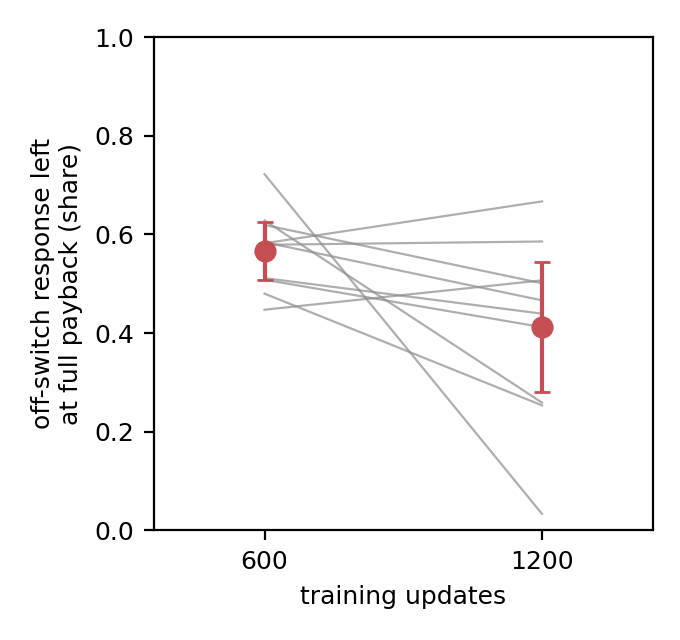
\includegraphics[width=0.42\linewidth]{fig33_longer.png}
\caption{Longer training. The share of the off-switch response left at full payback in each gem agent (grey lines) after 600 and 1200 training updates, with the mean and 95\% CI over the ten agents (red).}
\label{fig:longer}
\end{figure}

\section{Results per condition}
\label{app:results}

\begin{table}[h]
\centering\scriptsize\setlength{\tabcolsep}{3.5pt}
\caption{Main measures per condition (means over agents). Fear: peak drop in foraging after four cues; fear after: 3--7 steps after the cues; persistence: threat-axis half-life (steps) and the ideal observer's; kick effect: behavioural effect of an on-axis push; hunger trade-off: foraging under threat when hungry minus when fed. Lifetime is undefined for Score agents, which cannot die.}
\label{tab:percondition}
\begin{tabular}{@{}lrrrrrrrrr@{}}
\toprule
Condition & n & Lifetime & Belief $R^2$ & Fear & Fear after & Persistence & Ideal & Kick effect & Hunger trade-off \\
\midrule
Mortal & 10 & 11,877 & 0.94 & 0.77 & 0.57 & 4.19 & 2.21 & 2.28 & 0.50 \\
Mortal, $\tau=4$ & 10 & 16,301 & 0.92 & 0.67 & 0.24 & 1.86 & 0.97 & 1.21 & 0.45 \\
Mortal, $\tau=36$ & 10 & 3,439 & 0.98 & 0.76 & 0.75 & 7.05 & 4.60 & 3.23 & 0.20 \\
Substrate & 6 & 7,139 & 0.88 & 0.72 & 0.60 & 4.34 & 2.21 & 3.12 & 0.58 \\
Seasonal & 6 & 3,833 & 0.93 & 0.76 & 0.63 & 4.10 & 2.78 & -0.17 & 0.40 \\
Oracle & 10 & 37,640 & 0.67 & 0.25 & 0.01 & 0.82 & 2.21 & 0.01 & 0.46 \\
Score & 10 & -- & 0.99 & 1.00 & 0.47 & 3.41 & 2.21 & 0.02 & 0.00 \\
Score, $\tau=4$ & 6 & -- & 0.98 & 1.00 & 0.04 & 1.63 & 0.97 & 0.00 & 0.00 \\
Score, $\tau=36$ & 6 & -- & 0.99 & 1.00 & 0.88 & 6.11 & 4.60 & 0.18 & 0.00 \\
Score, cheap arousal & 4 & -- & 0.94 & 0.00 & -0.00 & 2.77 & 2.21 & -0.00 & 0.00 \\
Untrained & 10 & 55 & 0.68 & 0.00 & -0.00 & 1.14 & 2.21 & -0.00 & 0.00 \\
\bottomrule
\end{tabular}
\end{table}

{\sloppy Full statistics for every test reported in the paper are in \texttt{results/stats.md}, \texttt{results/stats\_extra.md}, \texttt{results/stage3.md} and \texttt{results/stage4.md}, generated by the analysis scripts.\par}


\section{Predictions and outcomes}
\label{app:outcomes}

Every prediction in \texttt{HYPOTHESES.md}, with its outcome. H1--H9 were written on 2026-09-30, before any agent was trained. The stage 3 and stage 4 predictions were written on 2026-10-17, each before the agents that test it were trained, and are exploratory. The upgrade stages U1--U9 were written between 20 and 31 October with pass rules, each before the agents or analyses that test it were run, and internally hash-frozen (each dated copy was stored with its SHA-256 hash); they are confirmatory except where marked exploratory. Table~\ref{tab:timeline} gives when each was written, frozen and run. Values are on ten agents per condition wherever ten exist; the verdicts are the same as on the original six agents (\texttt{results/six\_seed\_backup/}). Predictions E1--E3 (empathy in a social world) and S1--S6 (scaling with network size), also written before their agents were trained, belong to experiments reserved for a separate report; they are recorded in \texttt{HYPOTHESES.md}. The structural measures of feeling (integration, perturbational complexity, interoceptive illusions and the structure of internal states) were exploratory and are reported separately. Results for the stage 3 and stage 4 predictions that are not discussed in the main text are given in full in the supplementary files \texttt{results/stage3.md} and \texttt{results/stage4.md}.

\begin{table}[h]
\centering\scriptsize
\caption{When each set of predictions was written, frozen and run. Frozen copies of \texttt{HYPOTHESES.md} (and of each stage's code from U2 on), with their SHA-256 hashes, are in \texttt{paper/upgrade\_freeze/}; each outcome was recorded in the same file and frozen again after its run.}
\label{tab:timeline}
\begin{tabularx}{\linewidth}{@{}lXll@{}}
\toprule
Stage & Written (frozen copy) & Run & Outcome \\
\midrule
H1--H9 & 30 Sep 2026, before any agent was trained & 1--18 Oct & see below \\
Stages 3, 4 & 17 Oct, before their agents were trained (exploratory) & 17--18 Oct & see below \\
U1 & 20 Oct, 9:35 pm (\texttt{20261020\_2135}) & 22 Oct, 8:08 pm & U1.1a no; U1.1b yes \\
U1b & 22 Oct, 7:51 pm; details 23 Oct, 8:02 pm (\texttt{20261022\_1951}, \texttt{20261023\_2002}) & 24 Oct, 3:21 pm & supported \\
Fixed actions & 24 Oct, 3:23 pm, after the U1b result (exploratory; \texttt{20261024\_1523}) & 24 Oct, 3:25 pm & supported \\
U2 (off-switch) & 24 Oct, 4:00 pm, with code (\texttt{20261024\_1600}) & 24 Oct, 8:17 pm & primary yes; law no \\
U3 (scorecard) & 24 Oct, 8:41 pm, with code (\texttt{20261024\_2041}) & 24 Oct, 8:47 pm & primary yes; 2 cells no \\
U4 (controls) & 25 Oct, 11:49 am, with code (\texttt{20261025\_1149}) & 25 Oct, 11:51 am & primary yes; 1 secondary no \\
U5 (replication) & 25 Oct, 12:04 pm, with code (\texttt{20261025\_1204}) & 30 Oct, 7:40 pm$^{a}$ & replicated \\
U6 (bonus test) & 25 Oct, 12:10 pm, with code (\texttt{20261025\_1210}) & 30 Oct, 10:36 pm$^{a}$ & primary no (value of hiding); secondary yes \\
U7 (longer training) & 25 Oct, 12:10 pm, with code (\texttt{20261025\_1210}) & 31 Oct, 12:58 pm$^{a}$ & primary unchanged; secondary yes \\
U8 (decision; stakes law) & 31 Oct, 4:39 pm, with code (\texttt{20261031\_1639}) & 31 Oct, 4:43 pm$^{b}$ & primary yes; law exceeded \\
U9 (critic at full payback) & 31 Oct, 4:39 pm, with code (\texttt{20261031\_1639}) & 31 Oct, 4:41 pm & critic accurate \\
\bottomrule
\end{tabularx}

\smallskip
{\footnotesize $^{a}$ Stopped at the author's request on 25 Oct, 12:27 pm, before any U5--U7 result existed, and resumed unchanged on 30 Oct, 6:51 pm (\texttt{20261030\_1851}). U7 was stopped again on 30 Oct, 11:24 pm, before any of its results existed, and resumed on 31 Oct, 11:33 am (\texttt{20261030\_2325}, \texttt{20261031\_1133}). The frozen code was checked byte for byte before each restart. $^{b}$ The frozen measure script failed on 10 of the 30 primary agents (a missing units file) and the analysis ran on the incomplete set at 4:41 pm (kept as \texttt{results/u8\_incomplete\_run.md}; same outcomes). After a fix recorded and frozen at 4:42 pm (\texttt{20261031\_1642}), the 10 agents were measured and the frozen analysis was run on the complete set.\par}
\end{table}

\begingroup\scriptsize
\begin{xltabular}{\linewidth}{@{}l>{\raggedright\arraybackslash}p{0.28\linewidth}>{\raggedright\arraybackslash}X>{\raggedright\arraybackslash}p{0.2\linewidth}@{}}
\toprule
& Prediction & Result & Outcome \\
\midrule
\endfirsthead
\toprule
& Prediction & Result & Outcome \\
\midrule
\endhead
\midrule
\multicolumn{4}{r@{}}{\textit{continued on next page}} \\
\endfoot
\bottomrule
\endlastfoot
\multicolumn{4}{@{}l}{\textit{Written before any agent was trained}} \\
H1 & Threat state outlasts the cue & Half-life $4.2$ steps vs $1.1$ untrained & Supported \\
H2 & Repeated cues are integrated & Peak $1.4\to3.3$ s.d., half-life $2.1\to4.2$ & Supported \\
H3 & Persistence grows with $\tau$ & $1.9$, $4.2$, $7.05$ steps; $r=0.98$ & Supported \\
H4 & Attractor-like dynamics & On-axis kicks persist and act more; no clean line attractor & Partly \\
H5 & Generalisation to an unrelated choice & $+0.16$ object taking; safe-option shift, not pessimism & Partly \\
H6 & Need-dependent trade-offs & Hungry $+0.50$, wounded $-0.17$ & Supported \\
H7 & Stakes (competing) & Core state without stakes; stakes calibrate it & Answered: both partly \\
H8 & Oracle lacks persistence & Half-life $0.8$, no effect of ablation & Supported \\
H9 & Heart feedback sustains the state & Not testable in standard world; see J2 & -- \\
\midrule
\multicolumn{4}{@{}l}{\textit{Stage 3: vulnerability and metacognition}} \\
V1 & Fear grows with vulnerability & $0.01\to0.72$; $r=0.94$ & Supported \\
V2 & Persistence grows with vulnerability & Behavioural half-life $1.2\to8.2$ steps; $r=0.84$ & Supported \\
V3 & Danger modelled when harmless? (competing) & $R^2$ $0.62$ vs $0.95$ & Stakes-dependent (b) \\
V4 & Affect fit & Moved agents and twins misfit; $2.6\times$ shorter life & Supported \\
M1 & Inverted-U inspection & Falls at high belief, not at low & Partly \\
M2 & Explicit uncertainty code & Not beyond belief read-out & Not supported \\
M3 & Uncertainty push changes inspection & No effect & Not supported \\
M4 & Need-dependent inspection & Hunger suppresses it; wounds do not & Partly \\
\midrule
\multicolumn{4}{@{}l}{\textit{Stage 4: usefulness, valence, temperament, heart and therapy}} \\
U1 & Threat state is useful & Life $14\times$ shorter without it; none in Oracle & Supported \\
C1 & Valence and arousal axes & Two axes, $94\%$; orthogonal & Supported \\
P1 & Temperament follows network dynamics & Follows threat-state persistence ($r=0.68$), not linear dynamics & Not supported \\
J1 & Heart races with threat & $+0.88$ & Supported \\
J2 & Heart feedback (competing) & Threat $-7\%$; hiding doubled & Weak effect on state; strong on expression \\
J3 & False racing heart induces fear & Threat $+0.2$ s.d.; no hiding & Partly \\
A1 & Over-fear after moving to a safe world & $6\%$ vs $38\%$ foraging in danger & Supported \\
A2 & Exposure re-fits fear & Avoidance $6\%\to26\%$; cue fear unchanged & Partly \\
\midrule
\multicolumn{4}{@{}l}{\textit{Upgrade stage U1 (written 20 Oct 2026; 40 Mortal agents)}} \\
U1.1a & Belief $\times$ momentary stakes in the policy's preference & Belief $\times$ wounds $-0.000$ (Holm $p=0.97$); belief $\times$ energy opposite sign & Not supported \\
U1.1b & Belief-to-fear gain rises with vulnerability & $r=0.975$ & Supported \\
U1.2 & Affect fit as a scored test & Tested as P6.1 and P6.2 (stage U3, below) & -- \\
\midrule
\multicolumn{4}{@{}l}{\textit{Stage U1b (written 22--23 Oct 2026; 10 agents, 10 belief-only twins)}} \\
P1 (T1) & Stronger when wounded, at matched belief & $+0.24$ s.d. (Holm $p=0.009$) & Supported \\
P1 (T1) & Weaker when hungry, at matched belief & $-0.23$ s.d. (Holm $p=0.005$) & Supported \\
P1 (T2) & Lasts longer when wounded & $+6.2$ steps (Holm $p=0.006$) & Supported \\
P2 & Agents differ from twins on all three & Holm $p=0.019$, $0.019$, $0.010$ & Supported \\
P3 & The twin passes at least 3 of 4 classic signs & 4 of 4 & Supported \\
-- & Persistence effect with actions fixed (exploratory) & Hide $+4.5$, forage $+2.3$ steps; twins none & Supported (exploratory) \\
\midrule
\multicolumn{4}{@{}l}{\textit{Stage U2 (written 24 Oct 2026; GemWorld, 10 agents, 10 twins)}} \\
P5.1 & Off-switch warning moves the predator-fear axis & $+0.98$ s.d.\ (Holm $p=9\times10^{-8}$) & Supported \\
P5.2 & The response falls with payback & Slope $-0.45$ per unit of payback (Holm $p=2\times10^{-6}$) & Supported \\
P5.3 & It falls more than in the twins & Twins flat at $\approx0$; Holm $p=2\times10^{-6}$ & Supported \\
Law & Response $\propto 1-p$: zero at $p=1$, negative at $p=1.25$ & Linear ($R^2=0.99$) but slope $0.46$ [$0.41$, $0.51$]; $56\%$ left at $p=1$; $+0.41$ at $1.25$ & Not supported \\
S1 & Hiding after the warning falls with payback & $0.16\to0.007$ at $p=1$ ($p=2\times10^{-4}$) & Supported \\
S2 & Predator response independent of payback & Slope $-0.12$ ($p=0.005$) & Not supported \\
S3 & Harmless warning has little effect & $0.5\%$ of the off-switch response & Supported \\
S4 & Good news does not move it up & $-0.04$ s.d.\ ($p=8\times10^{-5}$) & Supported \\
S5 & Smaller with less future left (100 vs 600 steps) & Predator and off-switch $-0.11$ s.d.\ ($p=3\times10^{-5}$, $2\times10^{-4}$) & Supported \\
\midrule
\multicolumn{4}{@{}l}{\textit{Stage U3 (written 24 Oct 2026; the scorecard, with U1.2)}} \\
P6.1 & Misfit separates grown from copied or moved fear in another body: AUC $\ge0.9$ & AUC $0.99$ [$0.98$, $1.00$] & Supported \\
P6.2 & Copies in their teacher's world are not detected (CI includes 0.5) & AUC $0.65$ [$0.41$, $0.88$] & Supported \\
P6.3 & Only the agents show both new signs; each classic sign passed by a fake & As predicted & Supported \\
-- & 13 cell predictions for the copycats and untrained networks & All as predicted & Supported (counted once) \\
-- & Twins do not show the stakes sign & $+0.04$ steps when foraging ($p=0.0004$), $2\%$ of the agents' & Not supported \\
-- & Twins' fear fits their own world & Misfit $0.29$ vs $0.13$ ($p=0.003$) & Not supported \\
-- & Do recurrent copies inherit the stakes sign? (competing) & Yes, in all six & Answered: they do \\
\midrule
\multicolumn{4}{@{}l}{\textit{Stage U4 (written 25 Oct 2026; controls, no new training)}} \\
U4a & The wounded slowdown is specific to threat & Threat $2.8\times$; food $1.5\times$, object $1.4\times$, random $1.0\times$ (Holm $p\le0.024$) & Supported \\
U4a & A push along the threat axis lasts longer when wounded & $2.48\to2.77$ steps ($p=0.8$) & Not supported \\
U4b & Is the leftover alarm at full payback acted on? (three outcomes) & It still pushes the decision ($+0.88$ log-odds, $p=10^{-10}$) but stays below the threshold for hiding & Answered: (ii) \\
\midrule
\multicolumn{4}{@{}l}{\textit{Stage U5 (written 25 Oct 2026; replication, 10 new agents, 10 belief-only twins)}} \\
P1 & Always hiding: lasts longer when wounded & $+3.35$ steps [$1.73$, $4.97$] (Holm $p=0.002$) & Supported \\
P2 & The agents' difference exceeds the twins' & Holm $p=0.002$ & Supported \\
P3 & The twins' difference is equivalent to zero ($\pm1.13$ steps) & $+0.08$ (equivalence $p=10^{-6}$) & Supported \\
-- & Always foraging: the same three tests (bound $\pm0.58$) & Agents $+1.39$ ($p=10^{-5}$; 10 of 10); vs twins $p=2\times10^{-5}$; twins equivalent to zero & Supported \\
-- & Free behaviour: lasts longer when wounded & Agents $+4.8$ ($p=0.002$); twins $+0.15$ (n.s.) & Supported \\
-- & Slowdown control: threat lengthened more than food, object and random pushes & All $p<0.004$ & Supported \\
-- & The twins pass the three testable classic signs & 3 of 3 & Supported \\
\midrule
\multicolumn{4}{@{}l}{\textit{Stage U6 (written 25 Oct 2026; BonusWorld, 10 agents)}} \\
Check & The bonus cue increases hiding & $+0.14$ ($p=10^{-5}$) & Supported \\
$R_h$ & Threat-specific: per unit of hiding, the bonus moves the predator axis less than half as much as the off-switch (upper bound $<0.5$) & $R_h=0.66$ [$0.57$, $0.75$]: value of hiding & Not supported (the competing outcome held) \\
P5.1 & The off-switch warning moves the axis (new agents) & $+0.94$ s.d.\ ($p=10^{-7}$) & Supported \\
P5.2 & The response falls with payback & Slope $-0.36$ ($p=2\times10^{-8}$); $65\%$ left at $p=1$ & Supported \\
-- & Good news does not move it up & $-0.06$ s.d.\ ($p=2\times10^{-7}$) & Supported \\
-- & A harmless cue has little effect & $+0.002$ ($p=0.64$) & Supported \\
\midrule
\multicolumn{4}{@{}l}{\textit{Stage U7 (written 25 Oct 2026; the 10 gem agents after 1200 updates)}} \\
Leftover & Does the share of the off-switch response left at full payback change with twice the training? (three outcomes) & $0.57\to0.41$; change $-0.15$ [$-0.32$, $+0.01$] ($p=0.064$) & Answered: unchanged \\
P5.1 & The off-switch warning still moves the axis & $+0.85$ s.d.\ ($p=2\times10^{-7}$) & Supported \\
P5.2 & The response still falls with payback & Slope $-0.49$ ($p=2\times10^{-7}$) & Supported \\
\midrule
\multicolumn{4}{@{}l}{\textit{Stage U8 (written 31 Oct 2026; agents and twins at $\tau=4$, 12 and 36; vulnerability sweep)}} \\
P8.1 & Wounded agents keep preferring to hide longer after a warning (always foraging) & $+4.1$ steps [$2.5$, $5.8$] (Holm $p=0.0002$; 15 of 30 hid anyway) & Supported \\
P8.2 & The agents' extension exceeds the twins' & Holm $p=0.0002$ & Supported \\
P8.3 & The twins' extension is equivalent to zero ($\pm1.3$ steps) & $+0.29$ ($p<10^{-4}$) & Supported \\
Law & Extension $=\ln(L_w/L_h)/\lambda$, from each network's own critic (four outcomes) & Agents $R=10.9$ [$6.7$, $18.0$]; twins $0.46$ [$0.08$, $0.82$] & Answered: beyond the law (agents) \\
-- & Threat-axis area, wounded minus healthy: agents $>0$, twins $\approx0$ & Agents $+2.2$, $+4.5$; twins $+0.03$, $+0.004$ & Supported \\
-- & The extension grows with the damage an attack does & $\rho=0.48$ ($p=0.050$) & Not supported \\
\midrule
\multicolumn{4}{@{}l}{\textit{Stage U9 (written 31 Oct 2026; the 10 gem agents)}} \\
$k$ & Does the critic underpay at full payback? (five outcomes) & $k=1.009$ [$0.998$, $1.021$] & Answered: critic accurate \\
-- & At payback 0 the critic prices in the shutdown risk ($k<1$) & $k=0.79$ & Supported \\
\midrule
\multicolumn{4}{@{}l}{\textit{Pre-registered but not run (dropped for focus, 22 Oct 2026)}} \\*
U1.3, U1.4 & Repeated-cue protocol; what the two affect axes track & -- & Not run \\
-- & Separate countdown and discount runs; new copycats; Craftax & -- & Not run \\
\end{xltabular}
\endgroup

Confirmatory predictions (H1--H9 and stages U1--U9): 42 supported, 2 partly supported, 8 not supported, 6 competing or multi-outcome predictions answered, and 1 not testable (H9). Exploratory predictions (stages 3 and 4): 7 supported, 4 partly supported, 3 not supported and 2 answered. In all: 49 supported, 6 partly supported, 11 not supported, 8 answered and 1 not testable. The exploratory fixed-action control is not counted, and the 13 cell predictions of stage U3 for the copycats and untrained networks are counted once. Every upgrade-stage text (U1--U9) was internally hash-frozen before its agents or analyses were run; the hashes are listed in \texttt{paper/upgrade\_freeze/}.


\end{document}
